\section{Reweighting of simulated events} \label{sec:reweighting}

Simulated signal and background samples are corrected for various effects through reweighting procedures outlined in this section.

\subsection{Trigger efficiency reweighting}

\subsubsection{\ptmiss+\mht triggers}
The performance of the \ptmiss+\mht triggers is measured using single muon events. The
events are selected from the SingleMuon using the \texttt{HLT\_IsoMu27} (\texttt{HLT\_IsoMu24}) trigger for 2017 (2018), and the offline muon is required to be well-identified and have \pt larger than 40 GeV. The same selection is required as for the single-muon control region used in the final fit (cf. sec. ~\ref{sec:selection_cr_1m}):

\begin{enumerate}
\item Veto on additional leptons, photons, b jets, $\tau_{had}$ candidates.
\item $\Delta\phi(jet,\ptvecmiss)>0.5$ for the four leading jets with $\pt>30~\GeV$.
\item (Calo \ptmiss - PF \ptmiss) / recoil < 0.5
\item $M_{T}(\ell,\ptmiss) > 160~\GeV$.
\item Central AK4 jet with $\pt>100 GeV$, passing the tight jet ID.
\end{enumerate}

The efficiency is calculated as a function of the hadronic recoil \pt and is shown in Fig.~\ref{fig:hlteff_met}.
The trigger is found to be more than $95\%$ efficient for events with a recoil larger than $250~\GeV$, and more than $99\%$ efficient for events with a recoil larger than $375~\GeV$. The MC-to-data scale factor is found to be within $1\%$ of unity everywhere except for the lowest recoil bin at $250~\GeV$, where it is within $2\%$.

To investigate the stability of the measurement in single muon events, the same method is used to extract the efficiency from samples of double muon and single electron events. Again, an identical selection to the analysis control regions is used (cf. sec. ~\ref{sec:selection_cr_2m} and~\ref{sec:selection_cr_1e}), with the exception of requiring the leading muon \pt to be larger than 40~\GeV and omitting the \ptmiss cut in the electron region. The \HT-binned \texttt{WJets} and \texttt{DYJets} simulation samples are used. The resulting data-to-MC efficiency scale factors for all regions are shown in Fig.~\ref{fig:hltsf_met}. For 2017, a clear trend is present: The scale factor in dimuon events is larger in absolute terms then the one from the single muon region, and the scale factor from single electron events is the smallest. The difference between all regions is within $1\%$ relative to the single muon region. For 2018, no clear trend is observed above a recoil of $250~\GeV$: The scale factors from all three regions agree within the available statistical precision. Finally, the scale factors obtained form the single muon region are used to reweight the simulation. The difference to the other regions is taken into account by assigning an overall $1\%$ uncertainty.

\begin{figure*}[hbtp]\begin{center}
    \includegraphics[width=0.49\textwidth]{fig/efficiency/trigger/met/data_mc_comparison_1m_2017.pdf}
    \includegraphics[width=0.49\textwidth]{fig/efficiency/trigger/met/data_mc_comparison_1m_2018.pdf}
    \caption{MET trigger turn-on curve measured in single muon events as a function of hadronic recoil \pt in the 2017 and 2018 \texttt{SingleMuon} datasets and \HT-binned \texttt{WJets} simulation samples. The vertical blue line indicates a recoil value of $250~\GeV$, which is the requirement used in the analysis selection. The bottom panel shows the MC-to-data scale factor, with the blue horizontal lines indicating deviations of $1\%$ and $2\%$ from unity, respectively.}
    \label{fig:hlteff_met}
 \end{center}\end{figure*}

\begin{figure*}[hbtp]\begin{center}
    \includegraphics[width=0.49\textwidth]{fig/efficiency/trigger/met/sf_comparison_2017.pdf}
    \includegraphics[width=0.49\textwidth]{fig/efficiency/trigger/met/sf_comparison_2018.pdf}
    \caption{MC-to-data efficiency scale factors measured single muon events (`1m'), dimuon events (`2m') and single electron events (`1e'). For the single-lepton regions, the \HT-binned \texttt{WJets} are used, and the \HT-binned \texttt{DY} samples are used for the dimuon region. The bottom panel shows the ratio of the scale factors obtained from each individual region to the scale factor obtained from the single muon region. The vertical blue line indicates a recoil value of $250~\GeV$, which is the requirement used in the analysis selection, while the horizontal lines indicate deviations of $\pm1\%$ from unity.}
    \label{fig:hltsf_met}
 \end{center}\end{figure*}



\subsubsection{Photon trigger}
The photon trigger efficiency is measured using events from the JetHT dataset collected with the \texttt{HLT\_PFHT1050} trigger, which was fully unprescaled in 2017 and 2018~\footnote{The other, prescaled \texttt{HLT\_PFHTXXX} paths yield lower statistical precision.}. Events are selected in the same way as for the photon analysis control region (cf. sec.~\ref{sec:selection_cr_g}), except for the photon \pt, recoil and trigger requirements. The trigger efficiency $\epsilon$ is then determined as:

$$\epsilon(\texttt{HLT\_Photon200}) = \frac{\text{Offline selection \&\& \texttt{HLT\_PFHT1050} \&\& \texttt{HLT\_Photon200}}}{\text{Offline selection \&\& \texttt{HLT\_PFHT1050}}} $$

The resulting efficiency in data and \texttt{GJets} \HT-binned simulation is shown in Fig.~\ref{fig:hlteff_photon}. The trigger efficiency in data is larger than $95\%$ for a photon \pt of larger than $215~\GeV$, and larger than $99\%$ for photon \pt larger than $400~\GeV$. Between $250$ and $400~\GeV$, there is a slight inefficiency amounting to approximately $1\%$ at the most, with a larger amplitude in 2017 than in 2018. In both years, the turn-on behavior is almost immediate in simulated events, resulting in an MC-to-data scale factor almost entirely driven by the efficiency in data. The scale factor is within $1\%$ of unity for all bins except the lowest 2017 bin at $215\~GeV$, where is deviates from unity by about $4\%$.

Based on these results, the offline \pt cut for the photon in the photon control region is chosen to be $215~\GeV$.

\begin{figure*}[hbtp]\begin{center}
    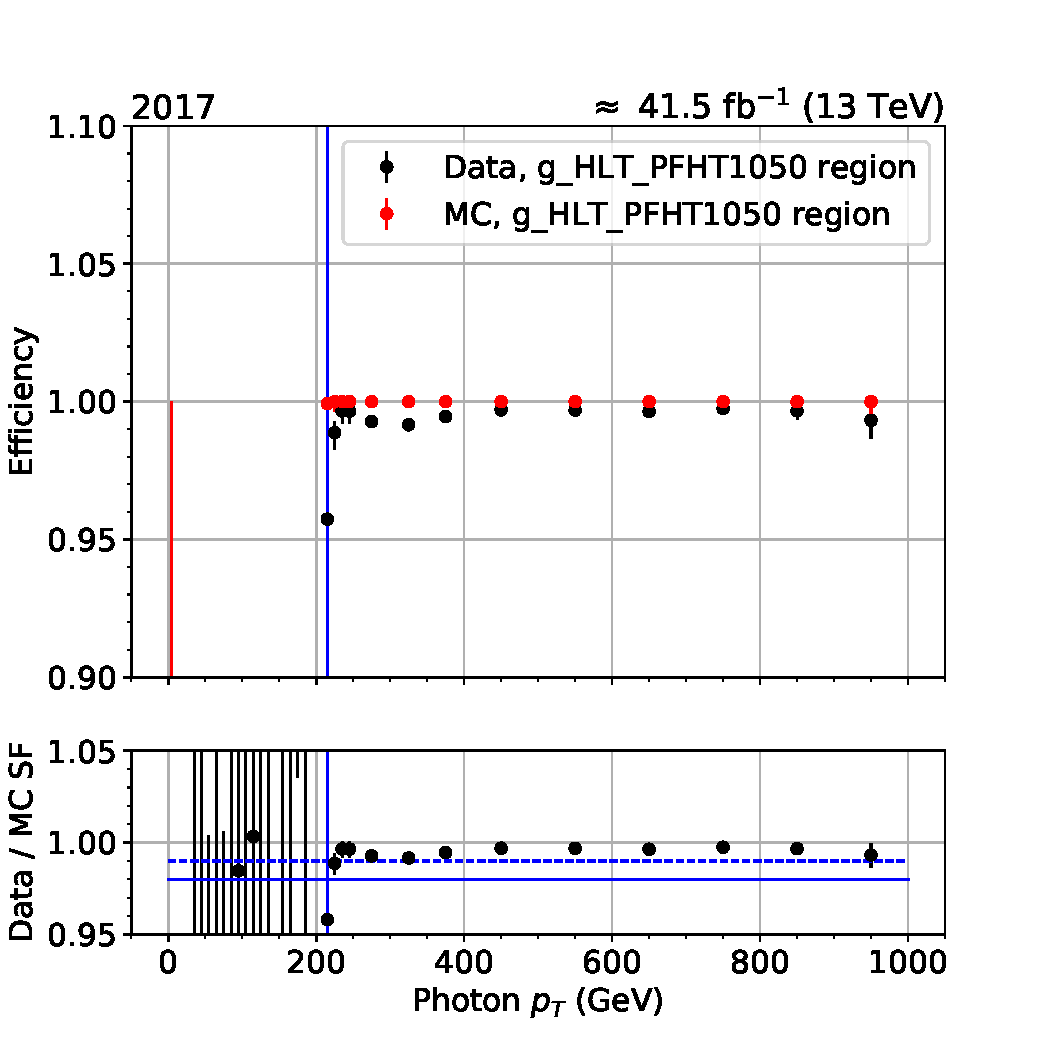
\includegraphics[width=0.49\textwidth]{fig/efficiency/trigger/photon/data_mc_comparison_g_HLT_PFHT1050_2017.pdf}
    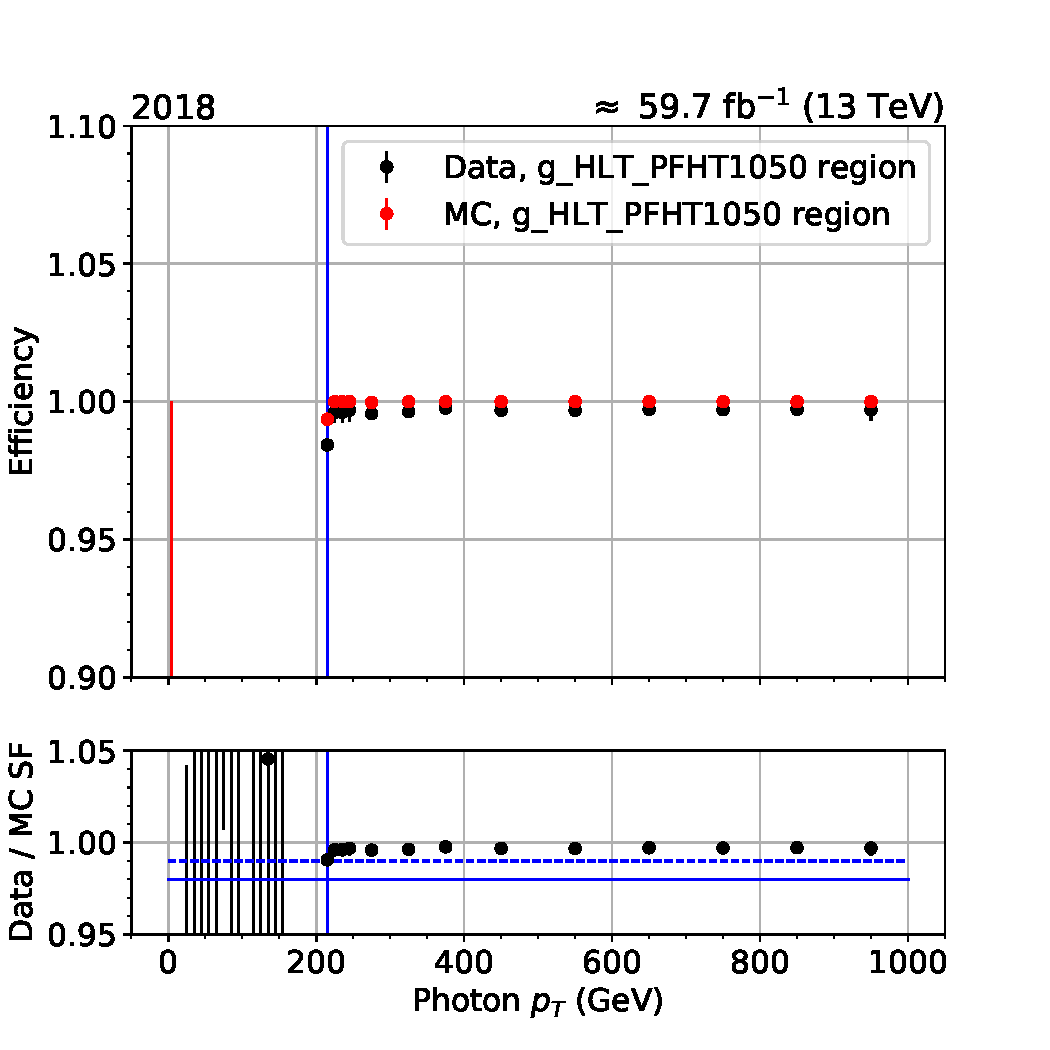
\includegraphics[width=0.49\textwidth]{fig/efficiency/trigger/photon/data_mc_comparison_g_HLT_PFHT1050_2018.pdf}
    \caption{Efficiency of the \texttt{HLT\_Photon200} trigger in data (black) and \HT-binned \texttt{GJets} simulation (red) for 2017 (left) and 2018 (right) as a function of photon \pt. The bottom panel shows the MC-to-data efficiency scale factor. The blue vertical line indicates a photon \pt of $215~\GeV$, which is the requirement used in the analysis selection.}
    \label{fig:hlteff_photon}
 \end{center}\end{figure*}

\subsubsection{Electron trigger}
{\color{red} We also need to add information about the single electron trigger efficiencies}

\subsection{Pileup reweighting}

The pileup (PU) conditions in the simulated samples are not identical to the ones observed measured in data, and a reweighting is applied to remove the difference.
The reweighting is performed by matching the true pileup distribution of each simulated sample
with the pileup distribution in data, obtained through the pileupCalc tool
assuming a minimum bias cross section of 69.2$\pm 4.6\%$~mb, following the recommendations in in Ref.~\cite{pileup_twiki}. The true pileup distributions in data and simulation are shown in Fig.~\ref{fig:purwg_true}. The distribution of the number of reconstructed vertices for $W\to \mu\nu$ events before and after PU reweighting is shown in Fig.~\ref{fig:purwt_npv}. In this variable, the PU reweighting method leads to a worse overall agreement between data and simulation. To check this behavior, the distribution of the event energy density $\rho$ is shown in Fig.~\ref{fig:purwt_npv}, again before and after PU reweighting. Here, the agreement before PU reweighting is worse than in the primary vertex distribution and the PU reweighting clearly improves the agreement.

\begin{figure}[ht!]
  \begin{center}
    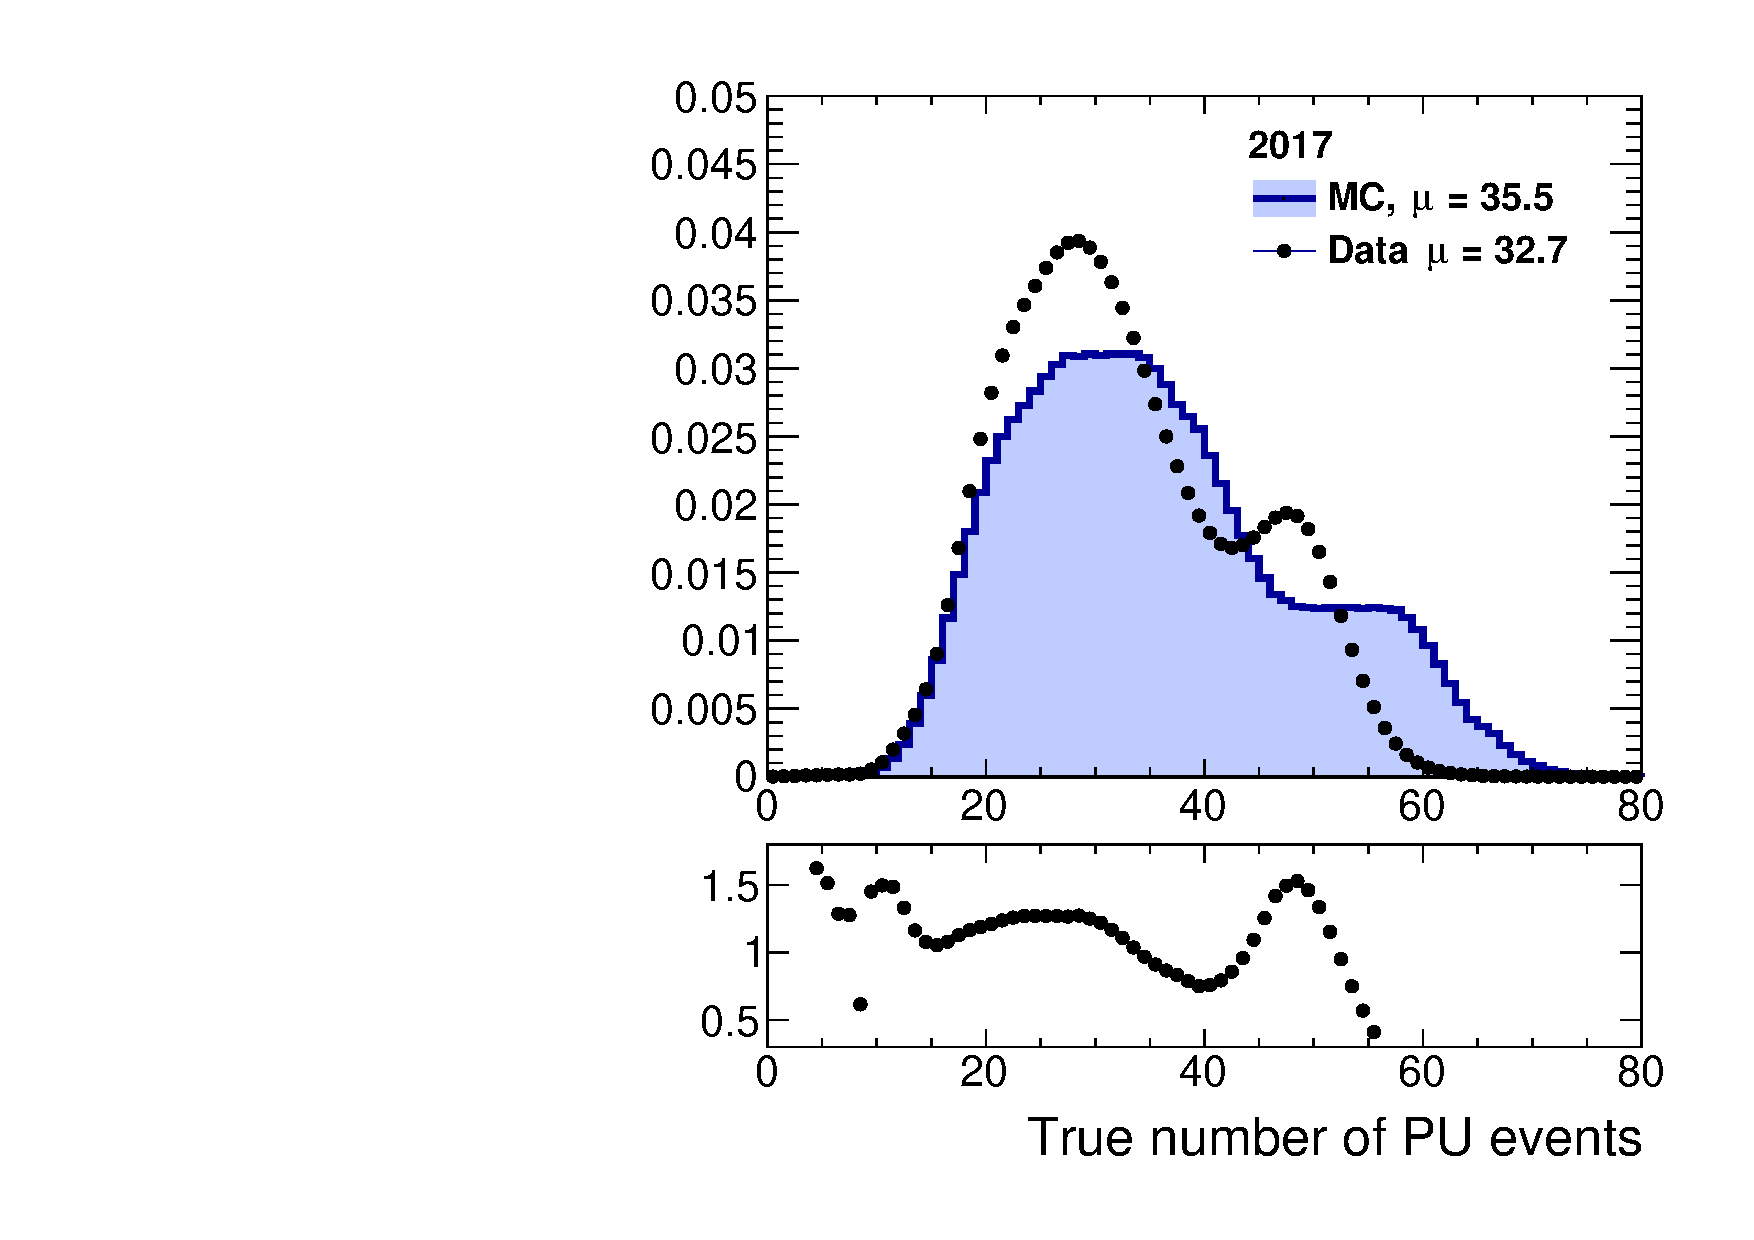
\includegraphics[width=0.49\textwidth]{fig/pileup/pu_weights_2017.pdf}
    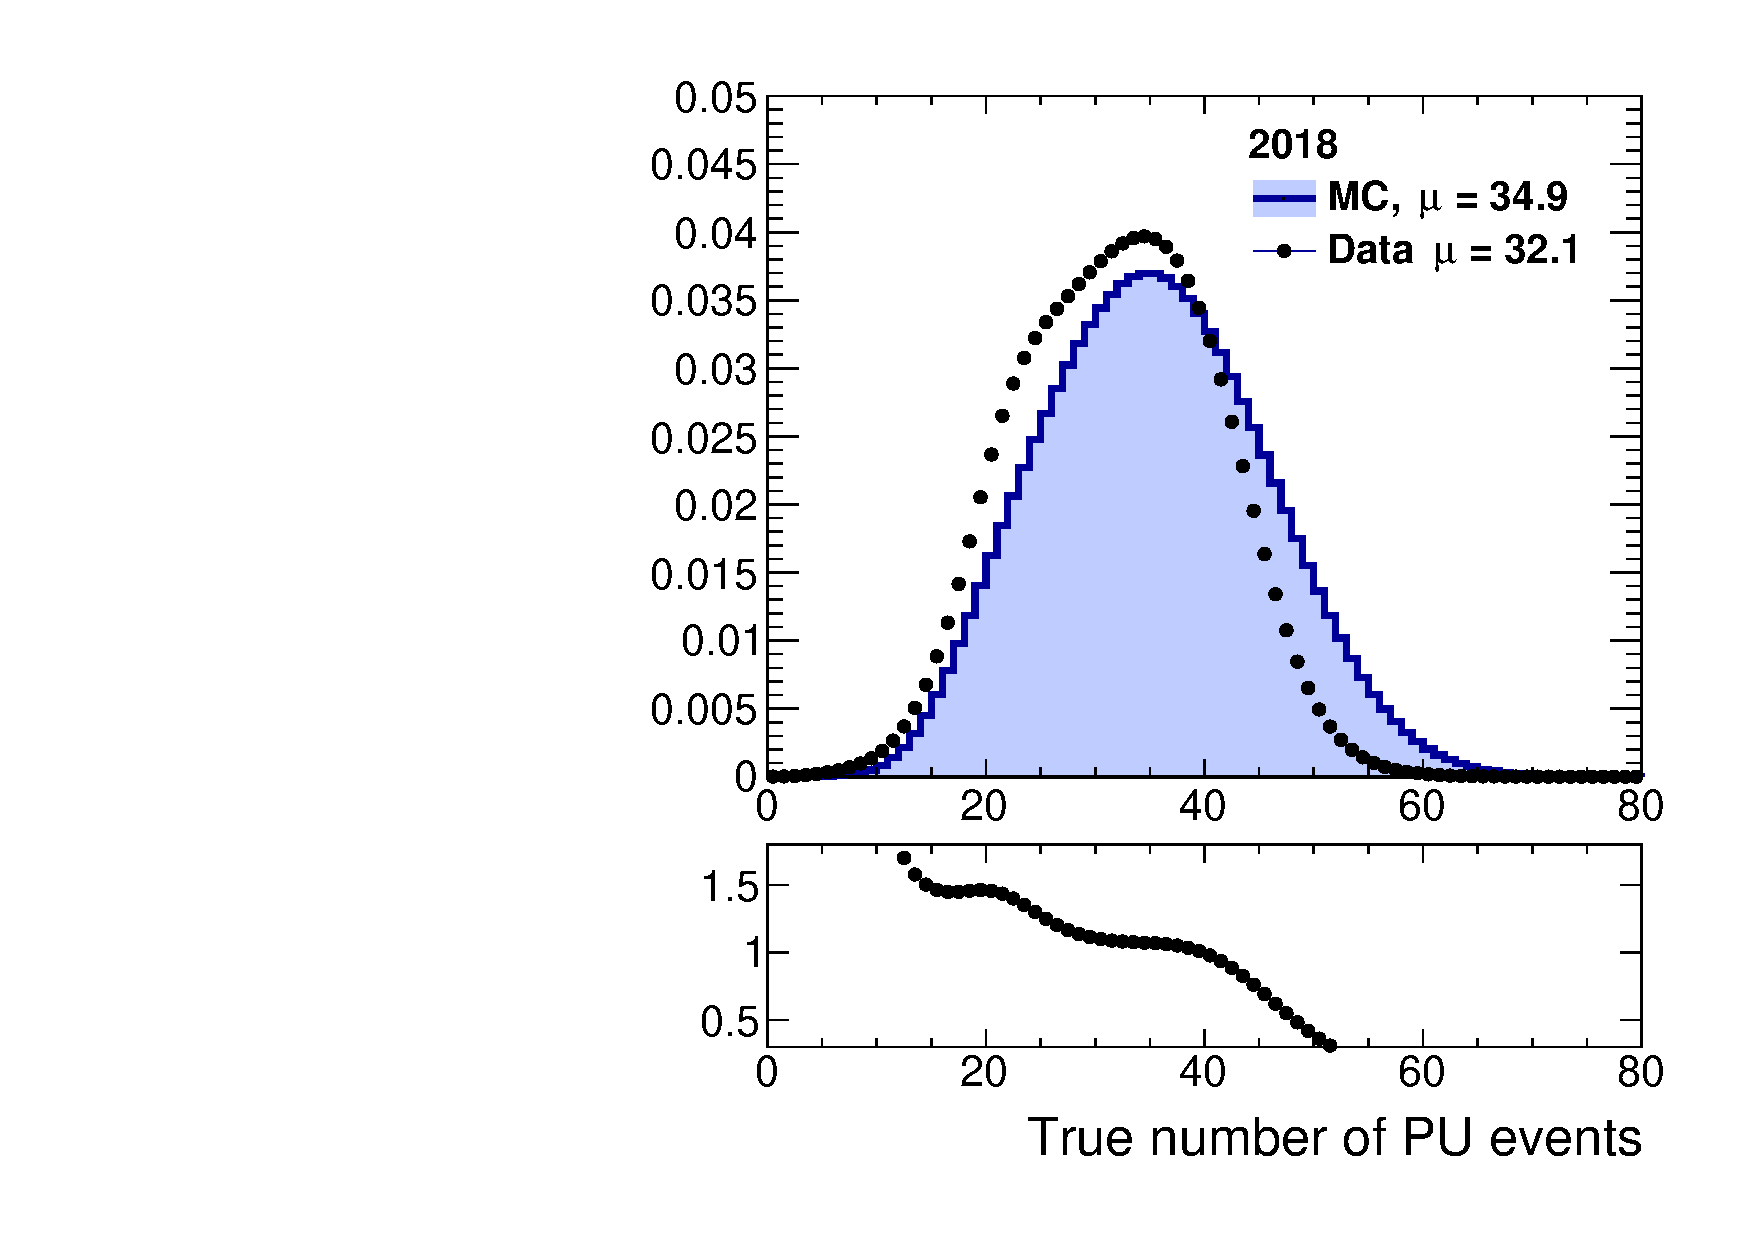
\includegraphics[width=0.49\textwidth]{fig/pileup/pu_weights_2018.pdf}
    \caption{
        Distribution of the true number of PU events in data and simulation for 2017 (left) and 2018 (right).
        The distributions for data are extracted assuming a minimum bias cross section of $69.2~\mathrm{mb}$.
    }
    \label{fig:purwg_true}
  \end{center}
\end{figure}
\begin{figure}[ht!]
  \begin{center}
    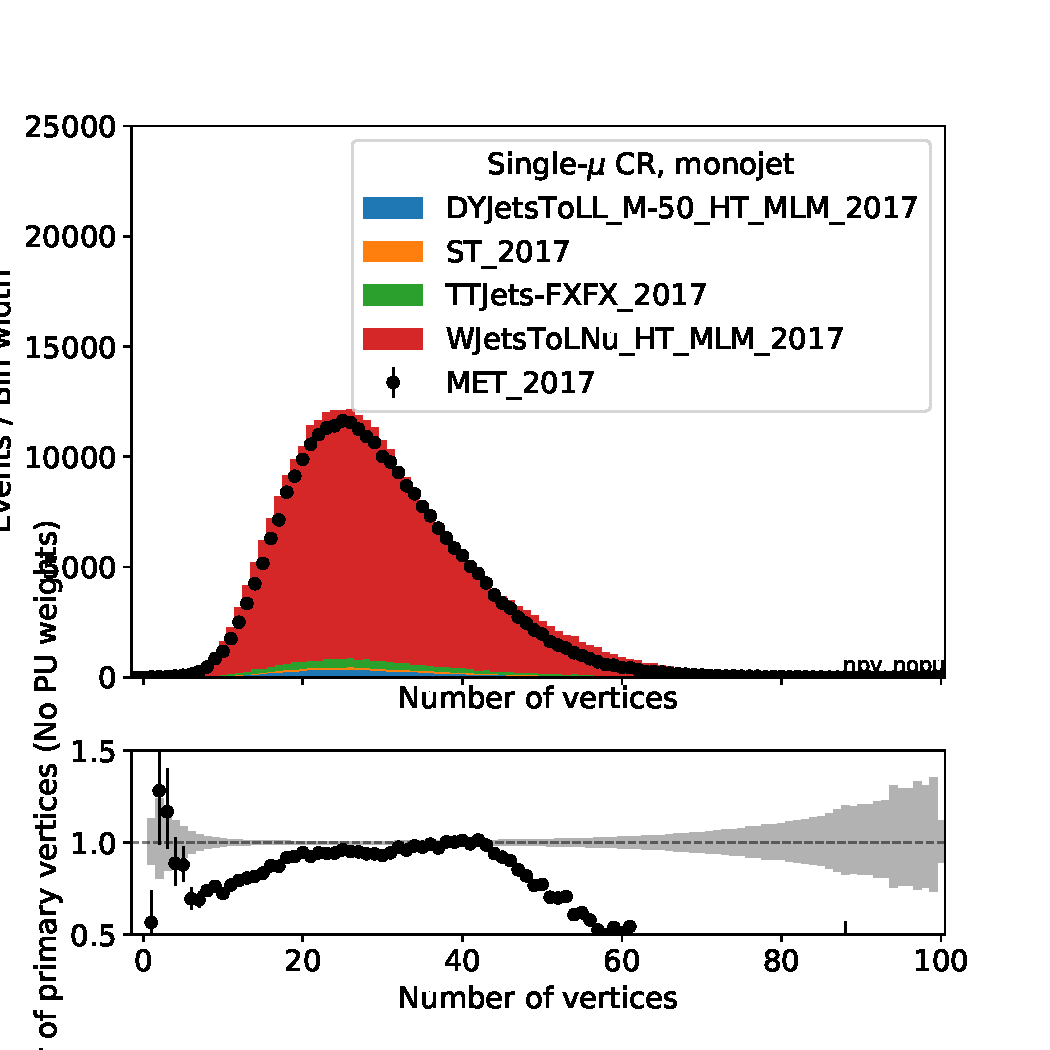
\includegraphics[width=0.49\textwidth]{fig/pileup/cr_1m_j_npv_nopu_2017.pdf}
    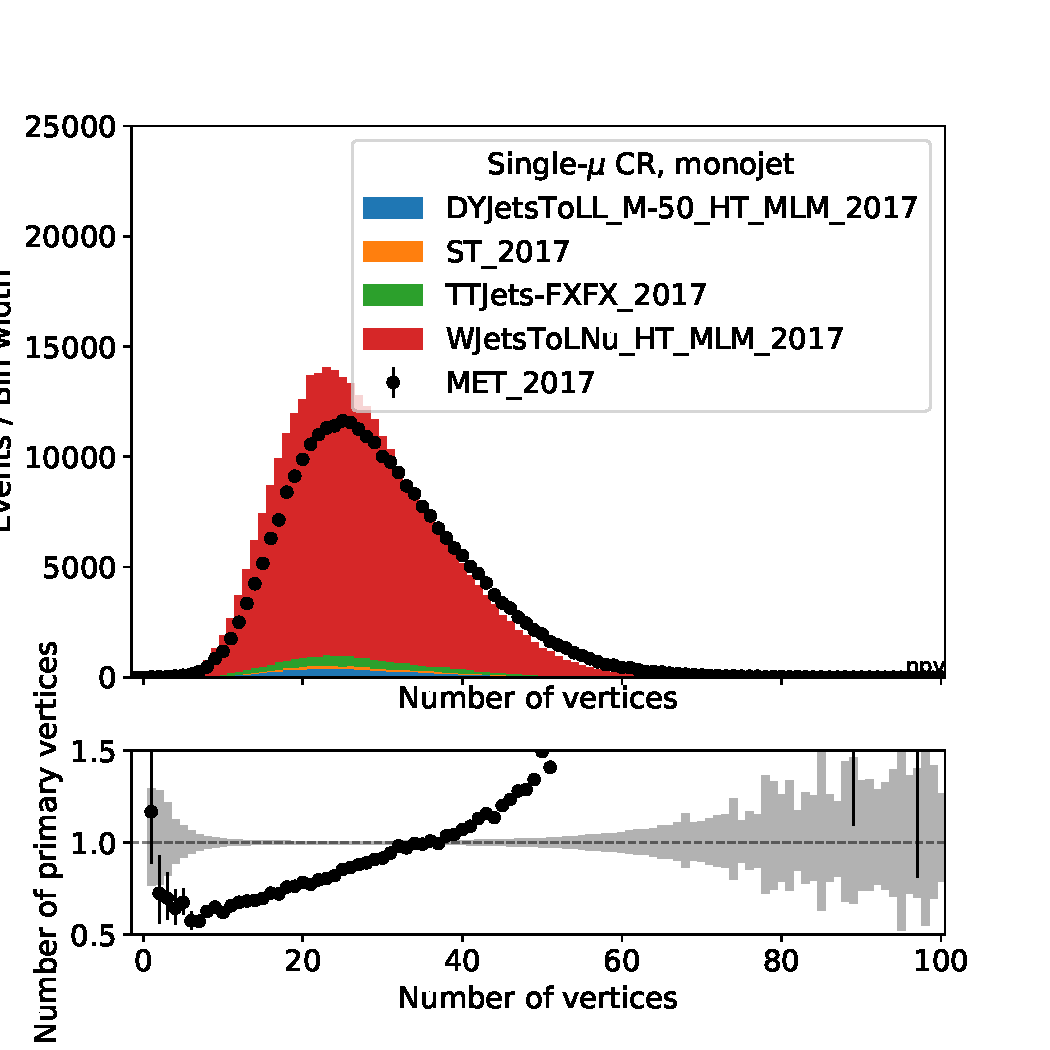
\includegraphics[width=0.49\textwidth]{fig/pileup/cr_1m_j_npv_2017.pdf}
    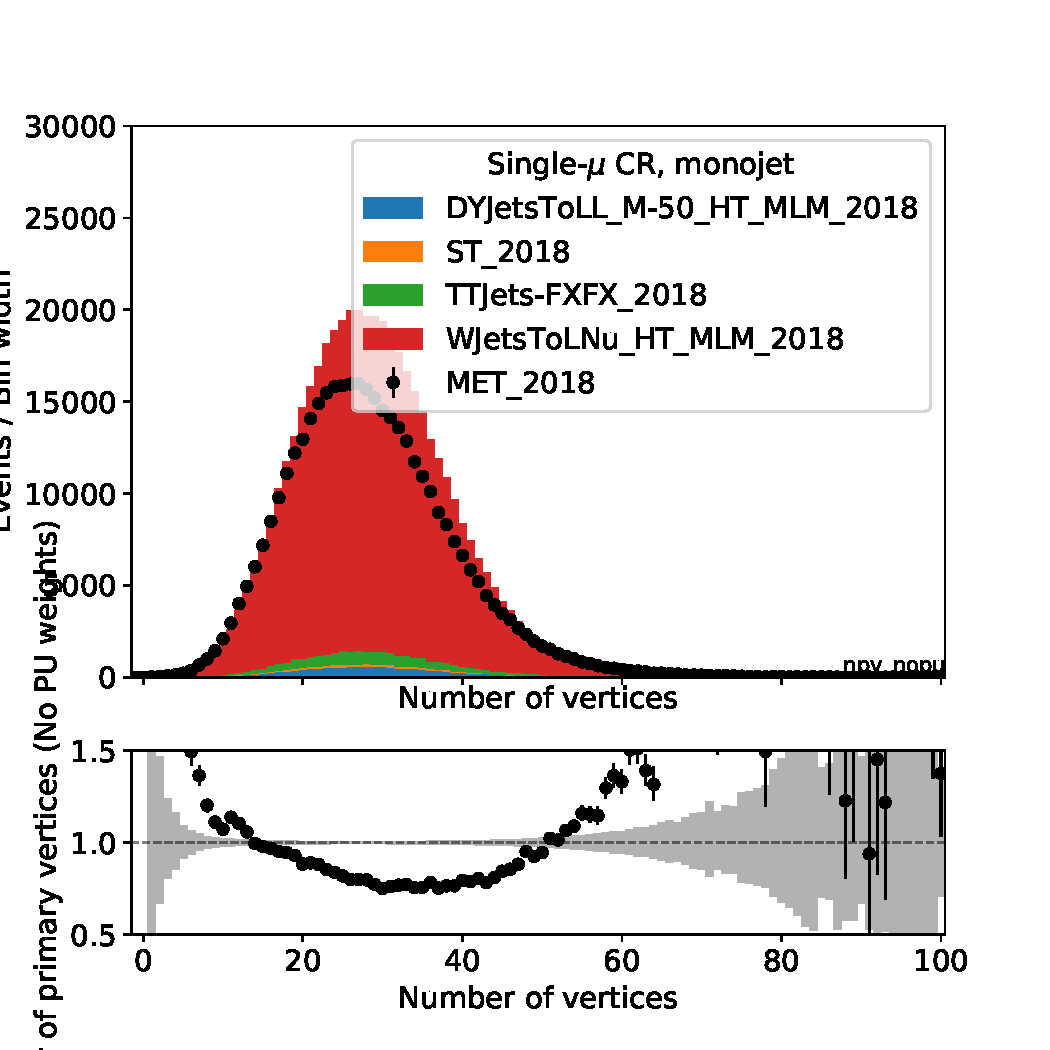
\includegraphics[width=0.49\textwidth]{fig/pileup/cr_1m_j_npv_nopu_2018.pdf}
    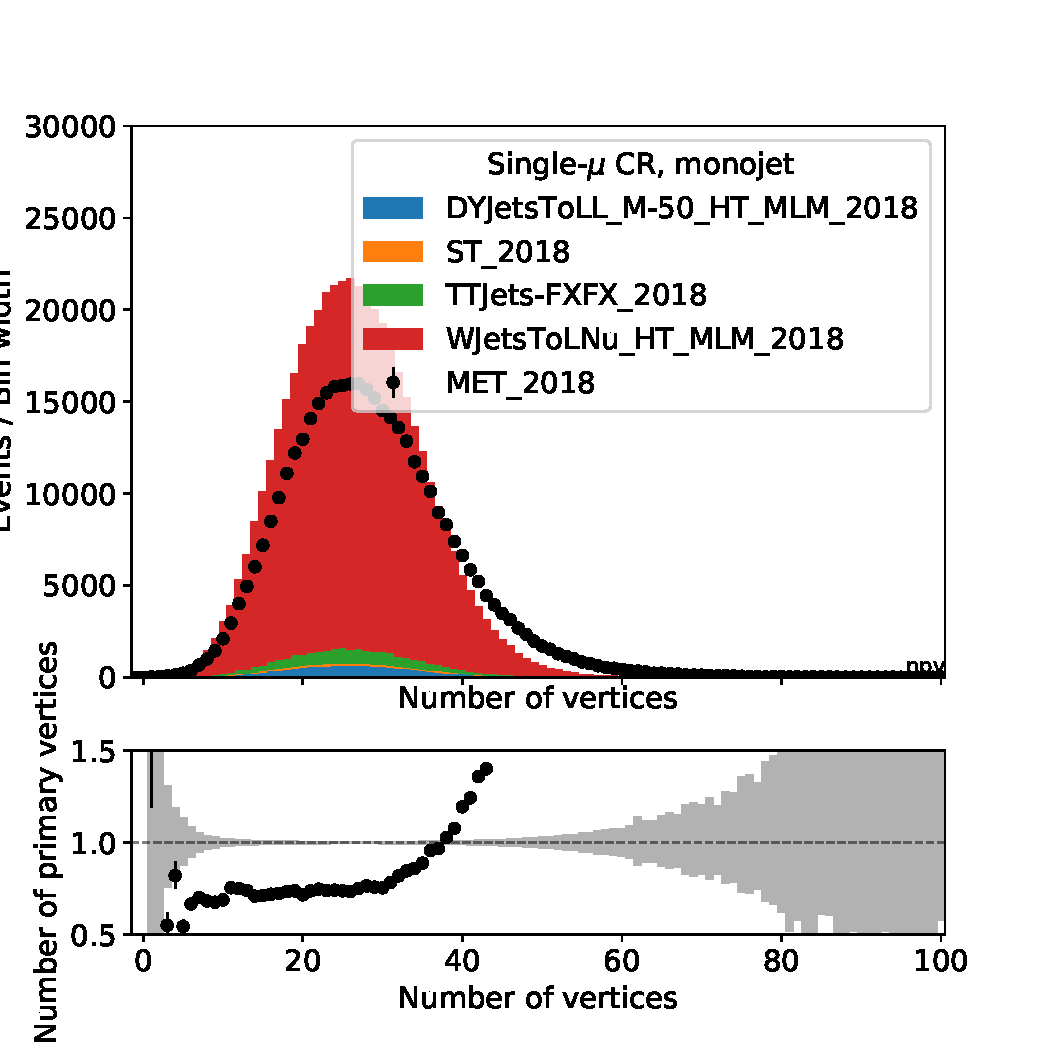
\includegraphics[width=0.49\textwidth]{fig/pileup/cr_1m_j_npv_2018.pdf}
    \caption{
        Distribution of the number of vertices in \Wmn~events in data and
        simulation before pileup re-weighting (left) and after pileup reweighting (right).
        The Monte Carlo is normalized to the luminosity of 41.53 and 59.7 fb$^{-1}$, respectively for 2017 and 2018.
    }
    \label{fig:purwt_npv}
  \end{center}
\end{figure}
\begin{figure}[ht!]
  \begin{center}
    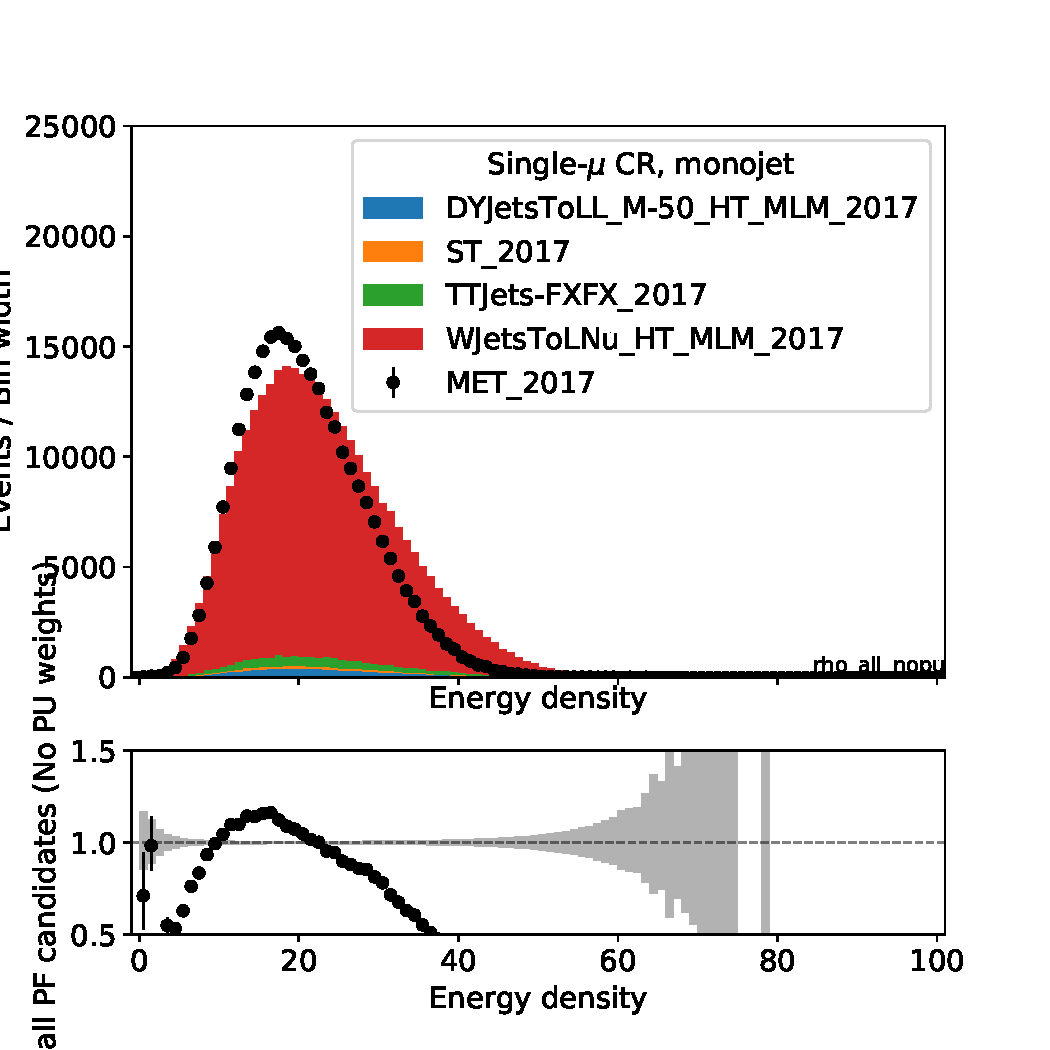
\includegraphics[width=0.49\textwidth]{fig/pileup/cr_1m_j_rho_all_nopu_2017.pdf}
    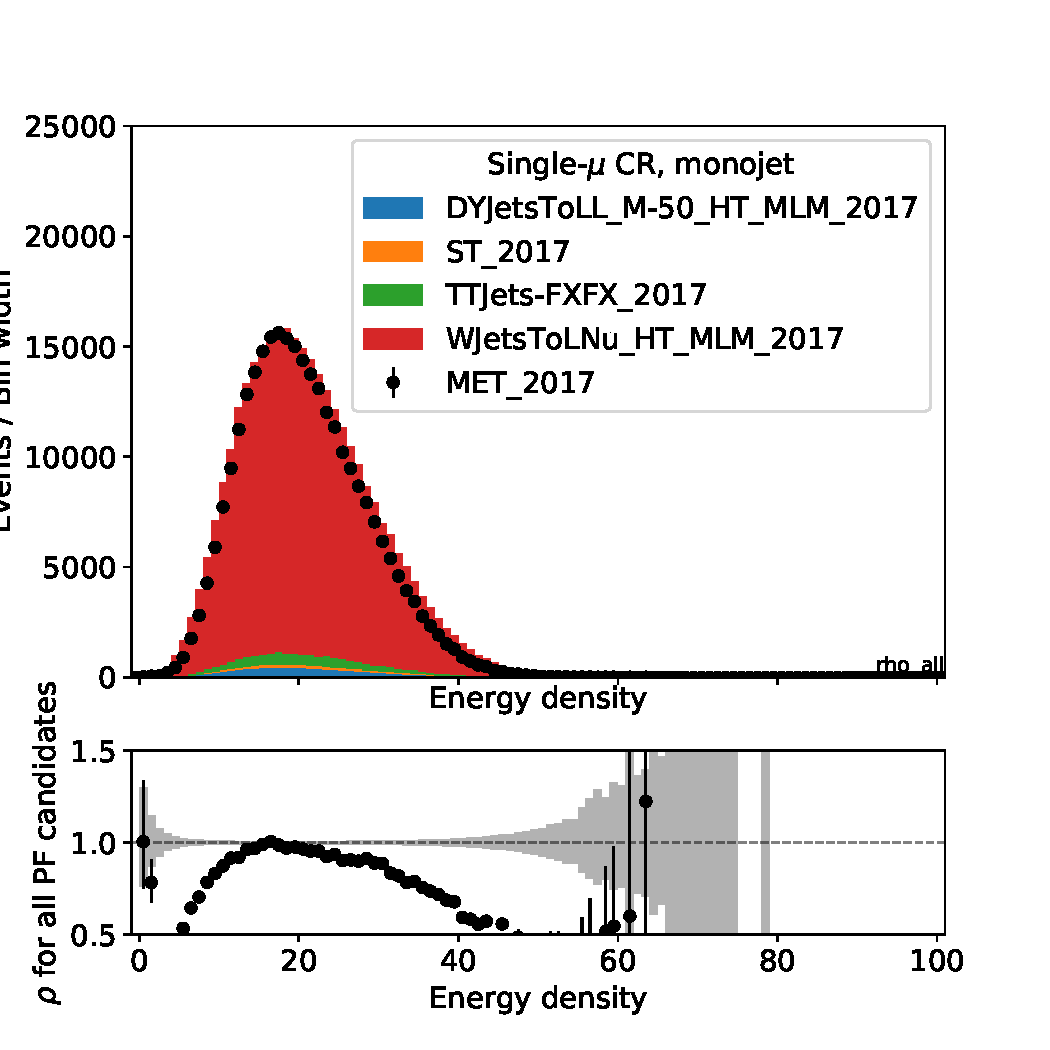
\includegraphics[width=0.49\textwidth]{fig/pileup/cr_1m_j_rho_all_2017.pdf}
    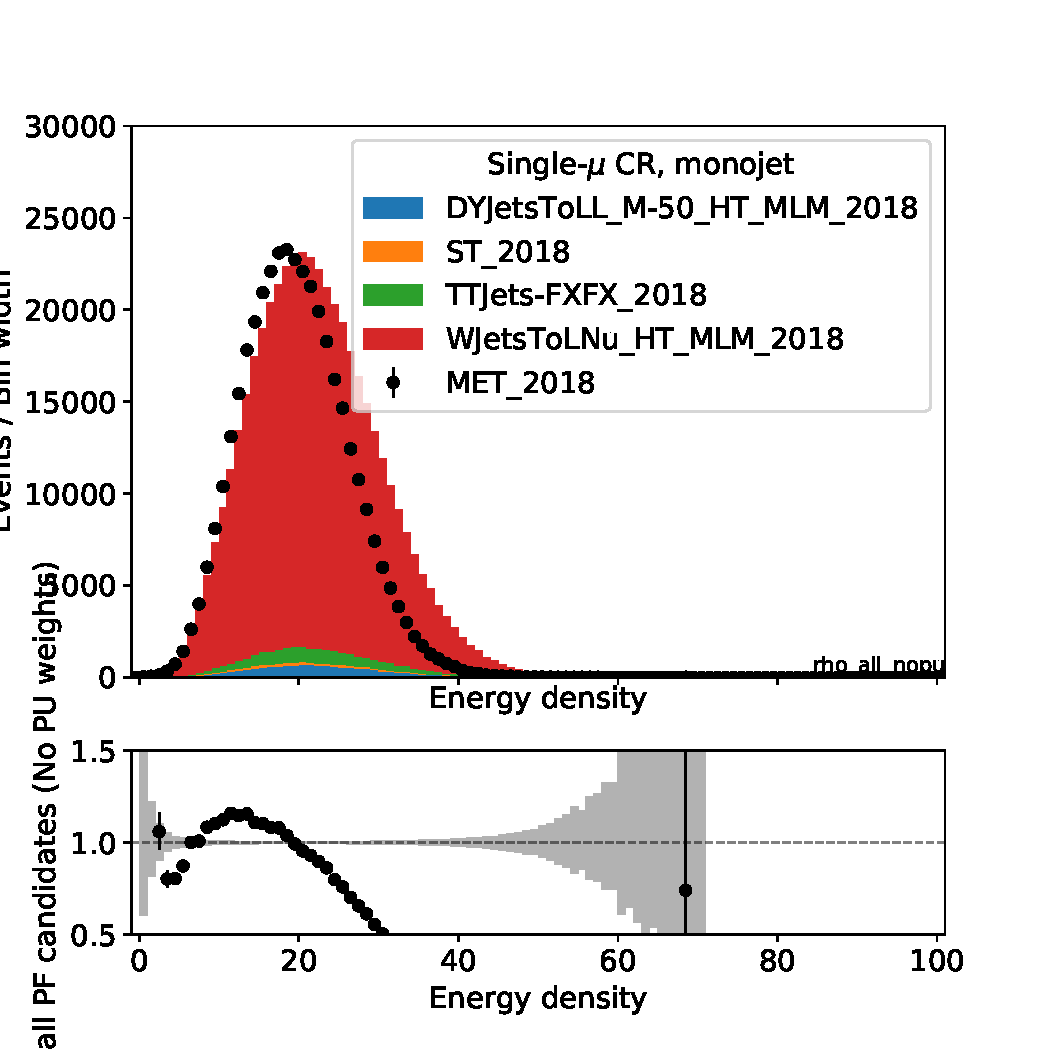
\includegraphics[width=0.49\textwidth]{fig/pileup/cr_1m_j_rho_all_nopu_2018.pdf}
    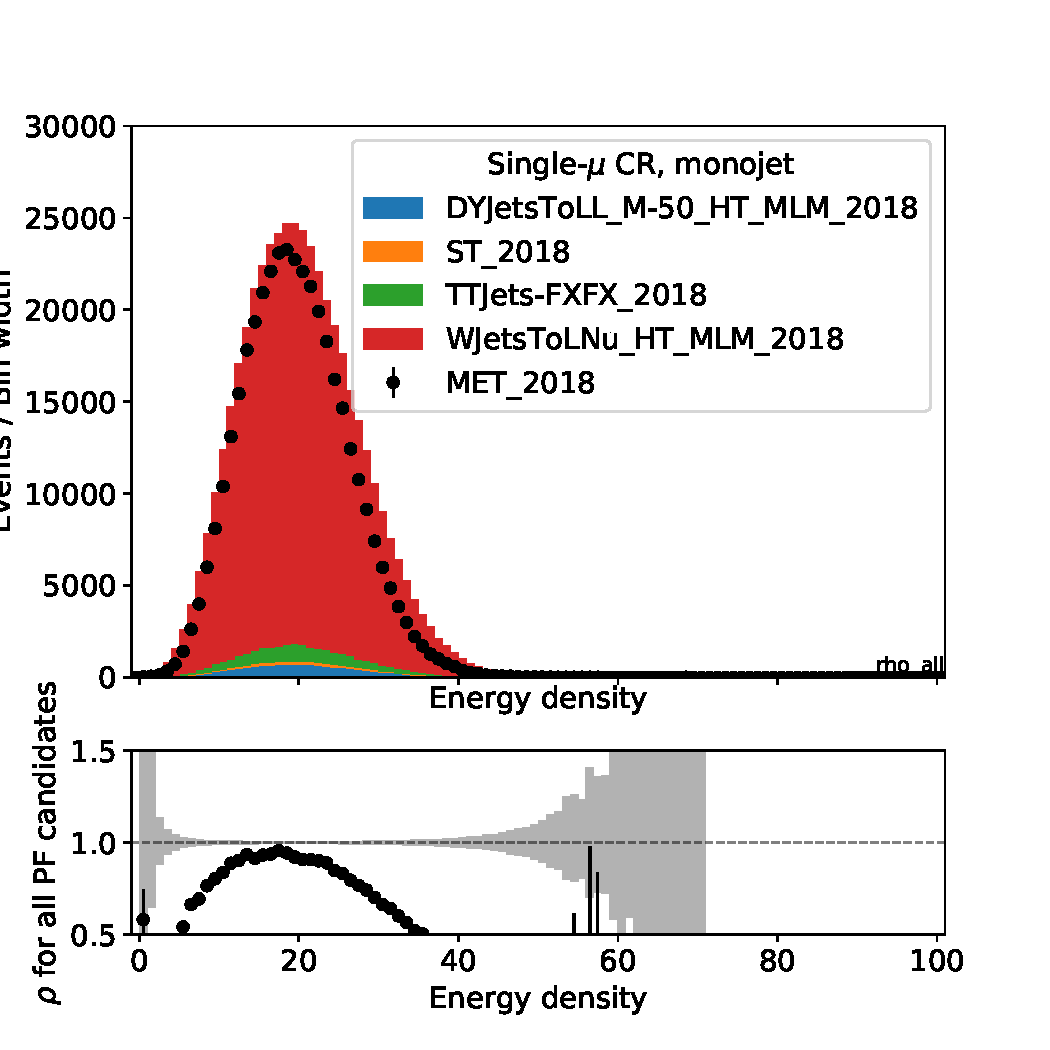
\includegraphics[width=0.49\textwidth]{fig/pileup/cr_1m_j_rho_all_2018.pdf}
    \caption{
        Distribution of the event energy density $\rho$  in \Wmn~events in data and
        simulation before pileup re-weighting (left) and after pileup reweighting (right).
        The Monte Carlo is normalized to the luminosity of 41.53 and 59.7 fb$^{-1}$, respectively for 2017 and 2018.
    }
    \label{fig:purwt_rho}
  \end{center}
\end{figure}

\subsection{Lepton and photon identification/reconstruction efficiency reweighting}

Data-to-simulation scale factors are applied to events in the control regions to
account for differences in the reconstruction, identification and isolation of leptons
between data and simulationn. These data-to-MC scale factors are derived from the efficiencies that are measured for the electron and muon
selections in bins of $\pt$ and $\eta$ in both data and simulation. These scale factors are
provided by the relevant POGs.


The reconstruction scale factors for electrons are shown in Fig.~\ref{fig:sf_electron_reco}. The corresponding identification scale factors for veto and tight electrons are shown in Fig.~\ref{fig:sf_electron_id}, and include the effect of the isolation efficiency. 

The identification scale factors for muons are shown in Fig.~\ref{fig:sf_muon_id}. Here, isolation scale factors are applied separately and are shown in Fig.~\ref{sf_muon_iso}. The corresponding corrections for muons are deemed negligible~\cite{CMS-MUO-TWIKI-SF}.

\begin{figure}[ht!]
  \begin{center}
    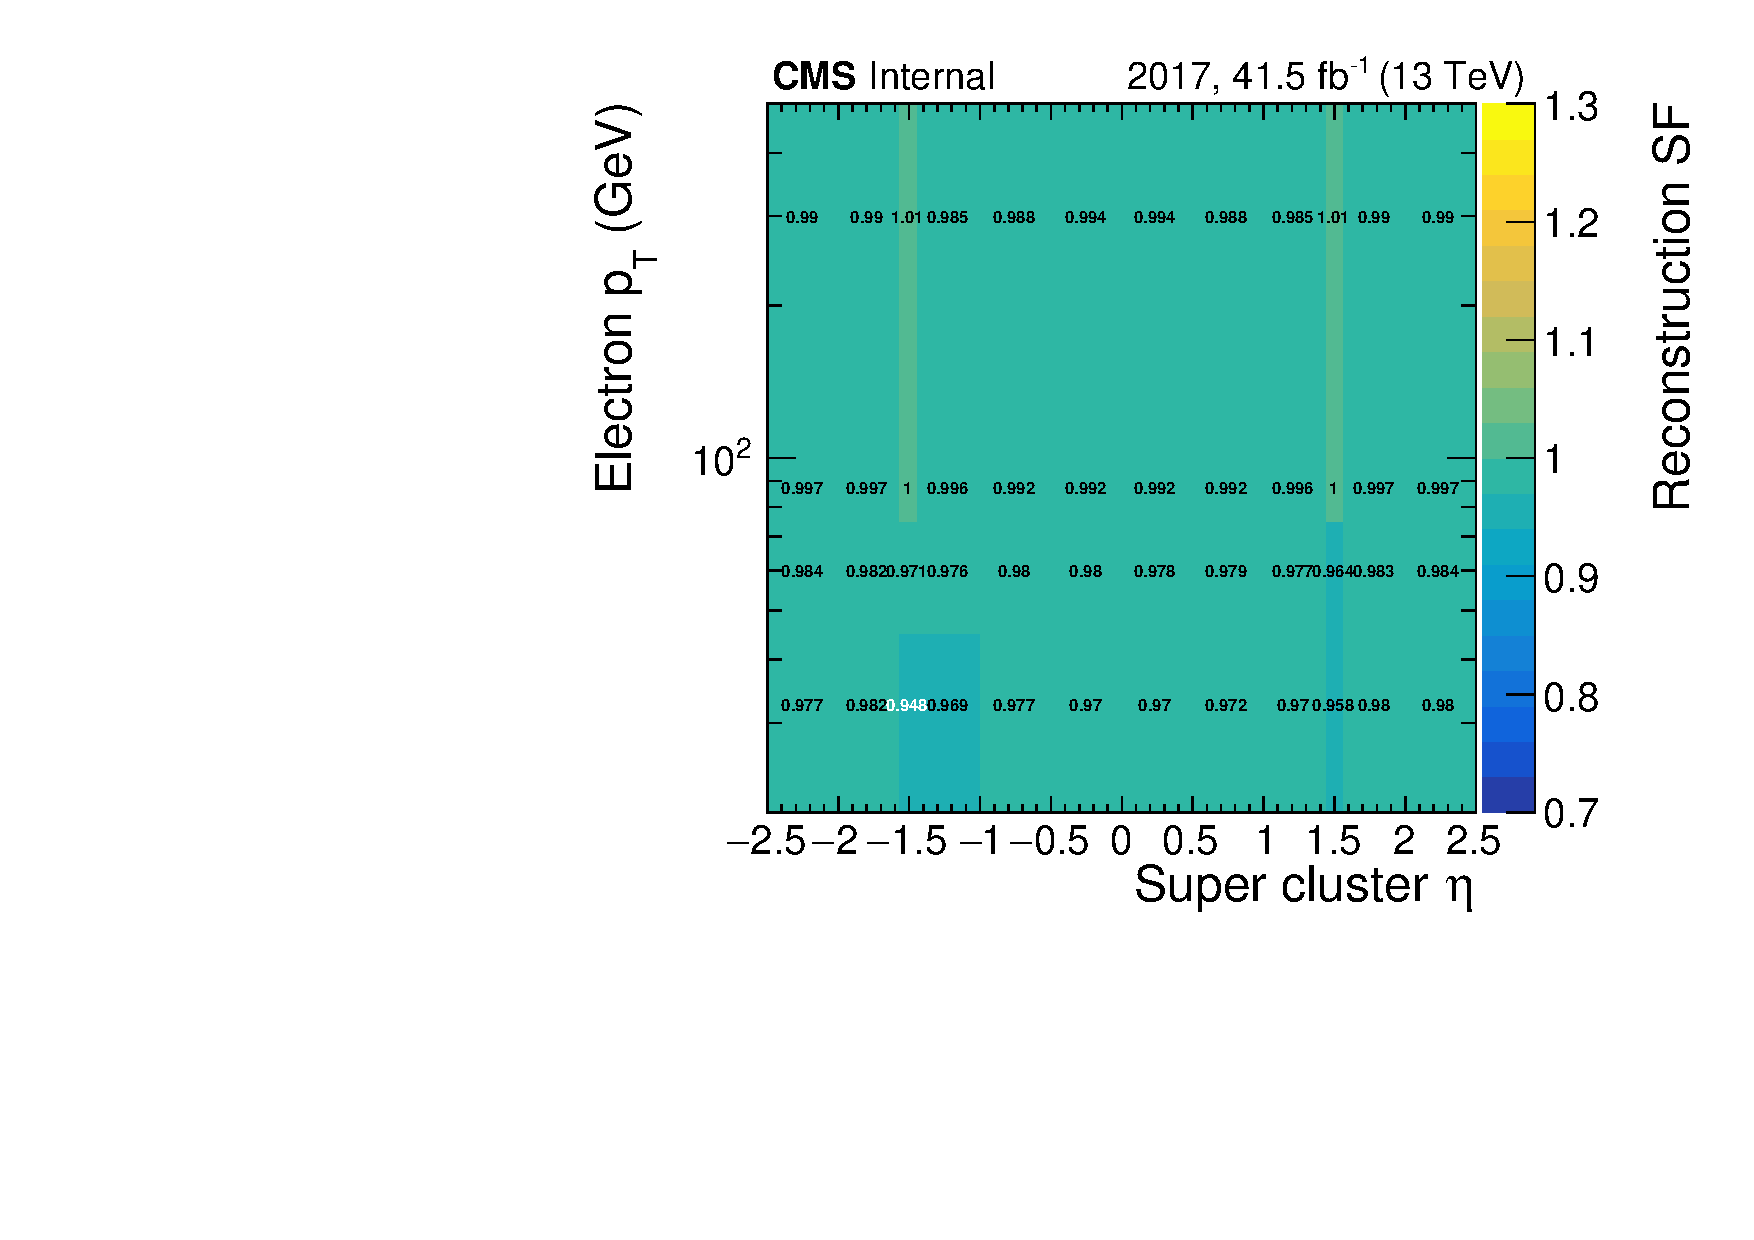
\includegraphics[width=0.49\textwidth]{fig/efficiency/lepton/ele_eff_reco_2017.pdf}
    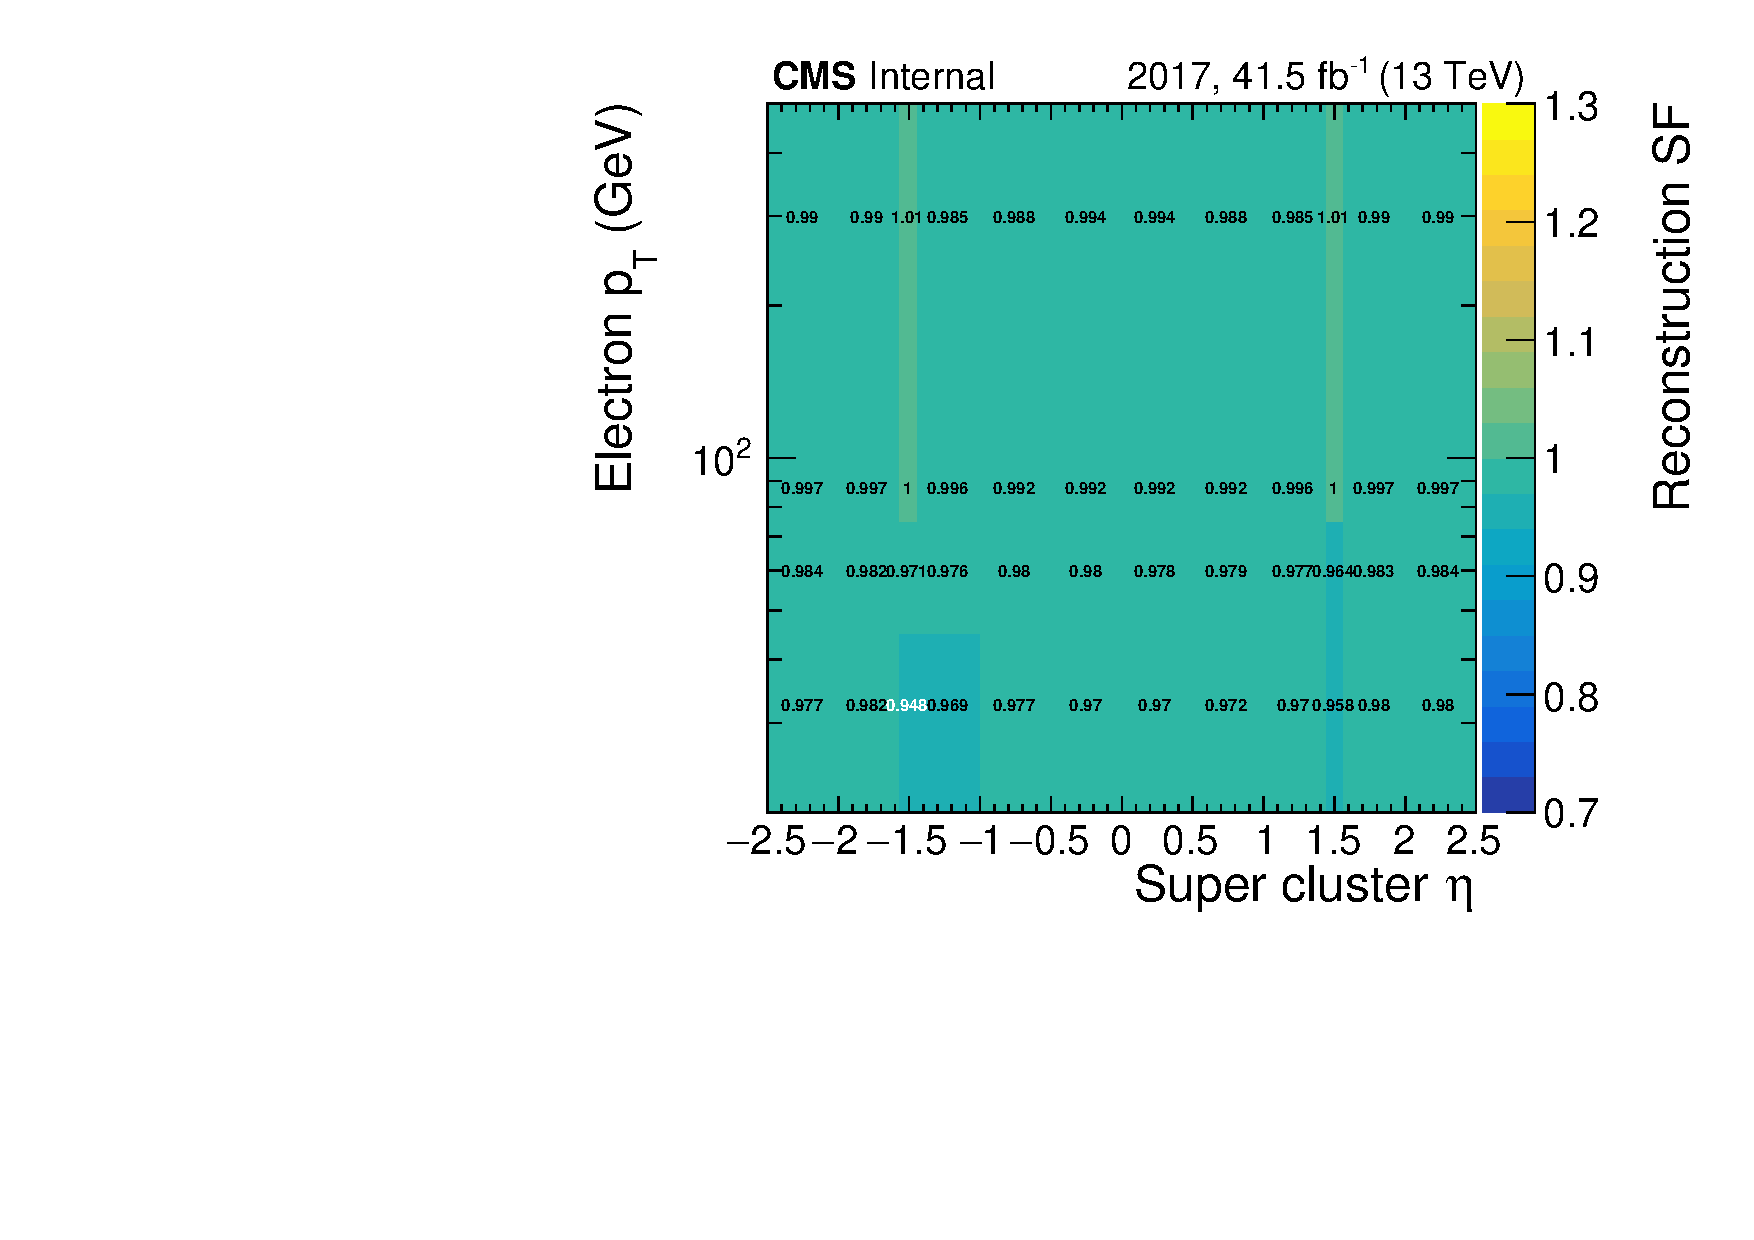
\includegraphics[width=0.49\textwidth]{fig/efficiency/lepton/ele_eff_reco_2017.pdf}\\
    \caption{
      Scale factors for the reconstruction efficiency of electrons starting from a super cluster for 2017 (left) and 2018(right)
    }
    \label{fig:sf_electron_reco}
  \end{center}
\end{figure}
\begin{figure}[ht!]
  \begin{center}
    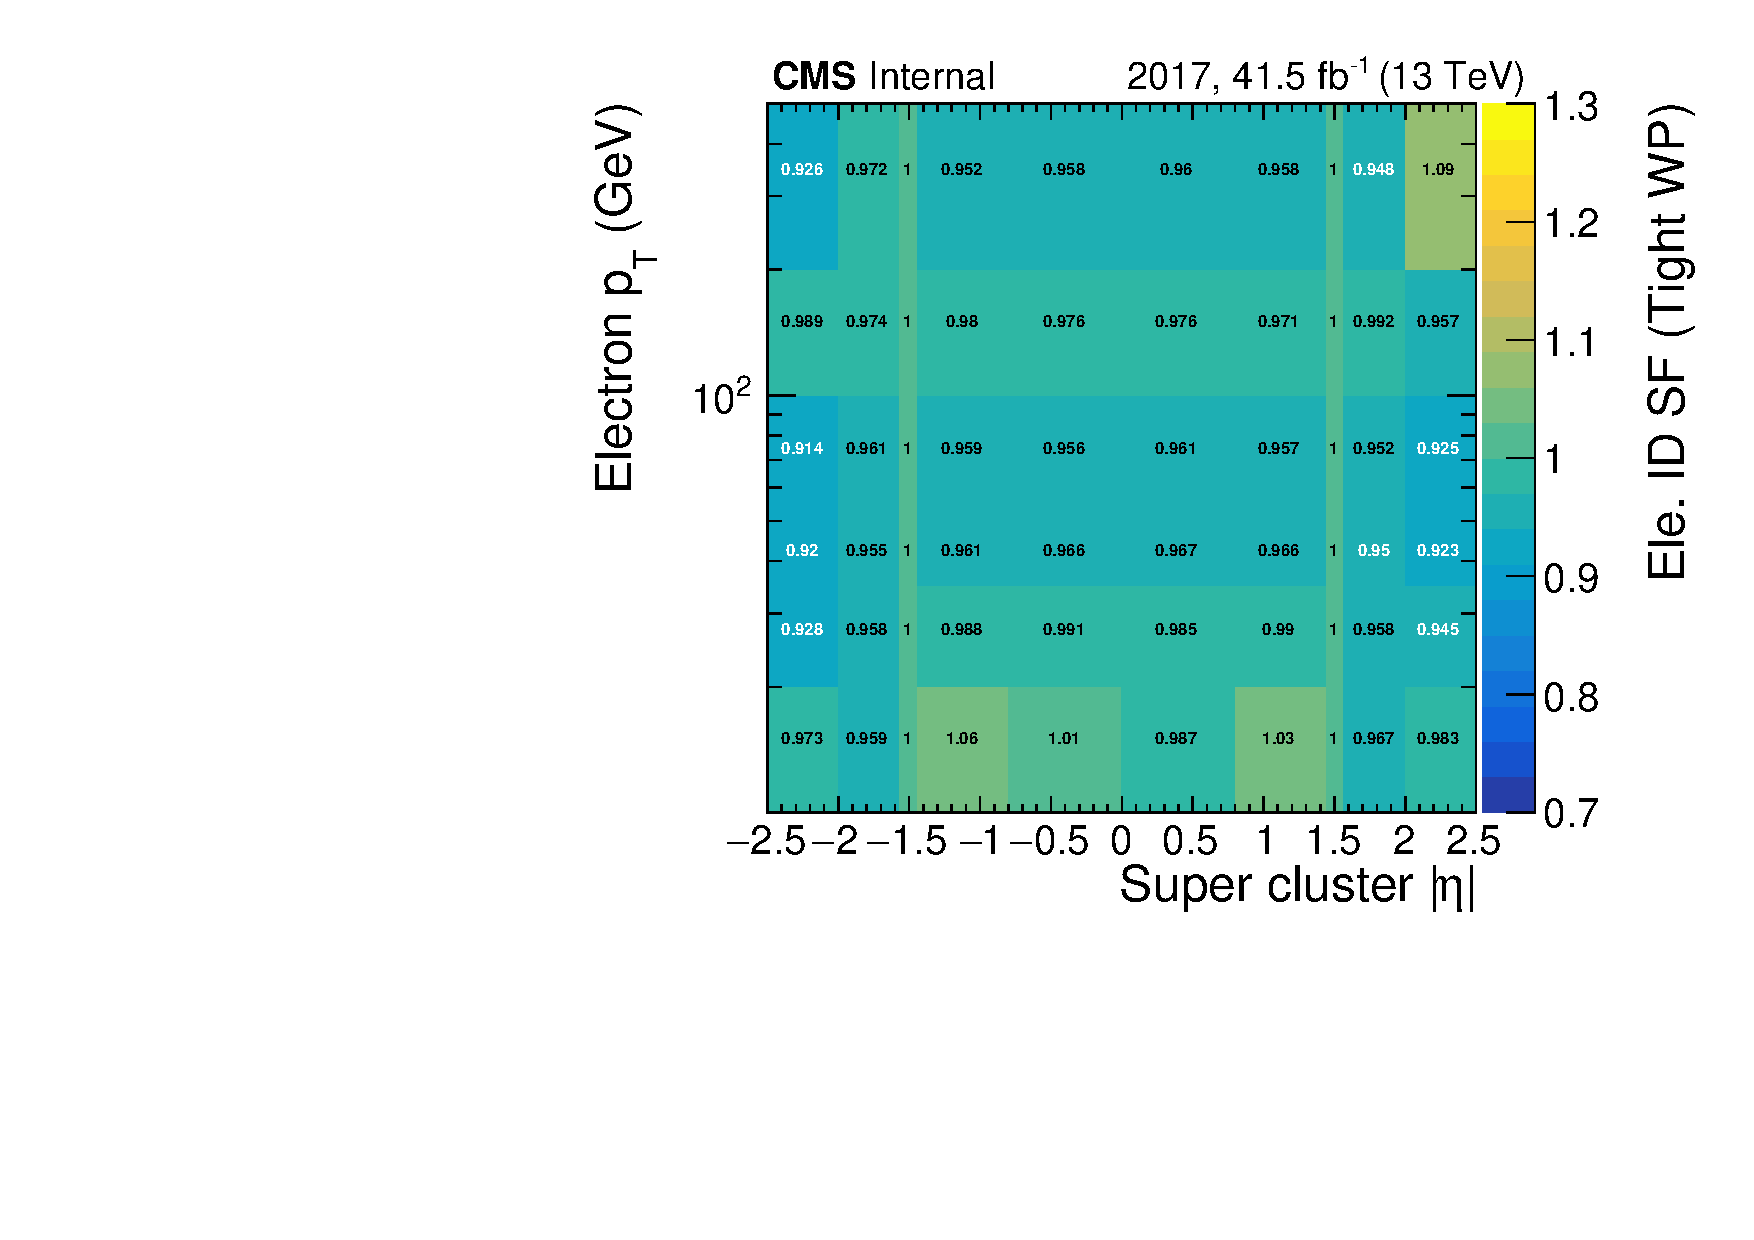
\includegraphics[width=0.49\textwidth]{fig/efficiency/lepton/ele_eff_tight_id_2017.pdf}
    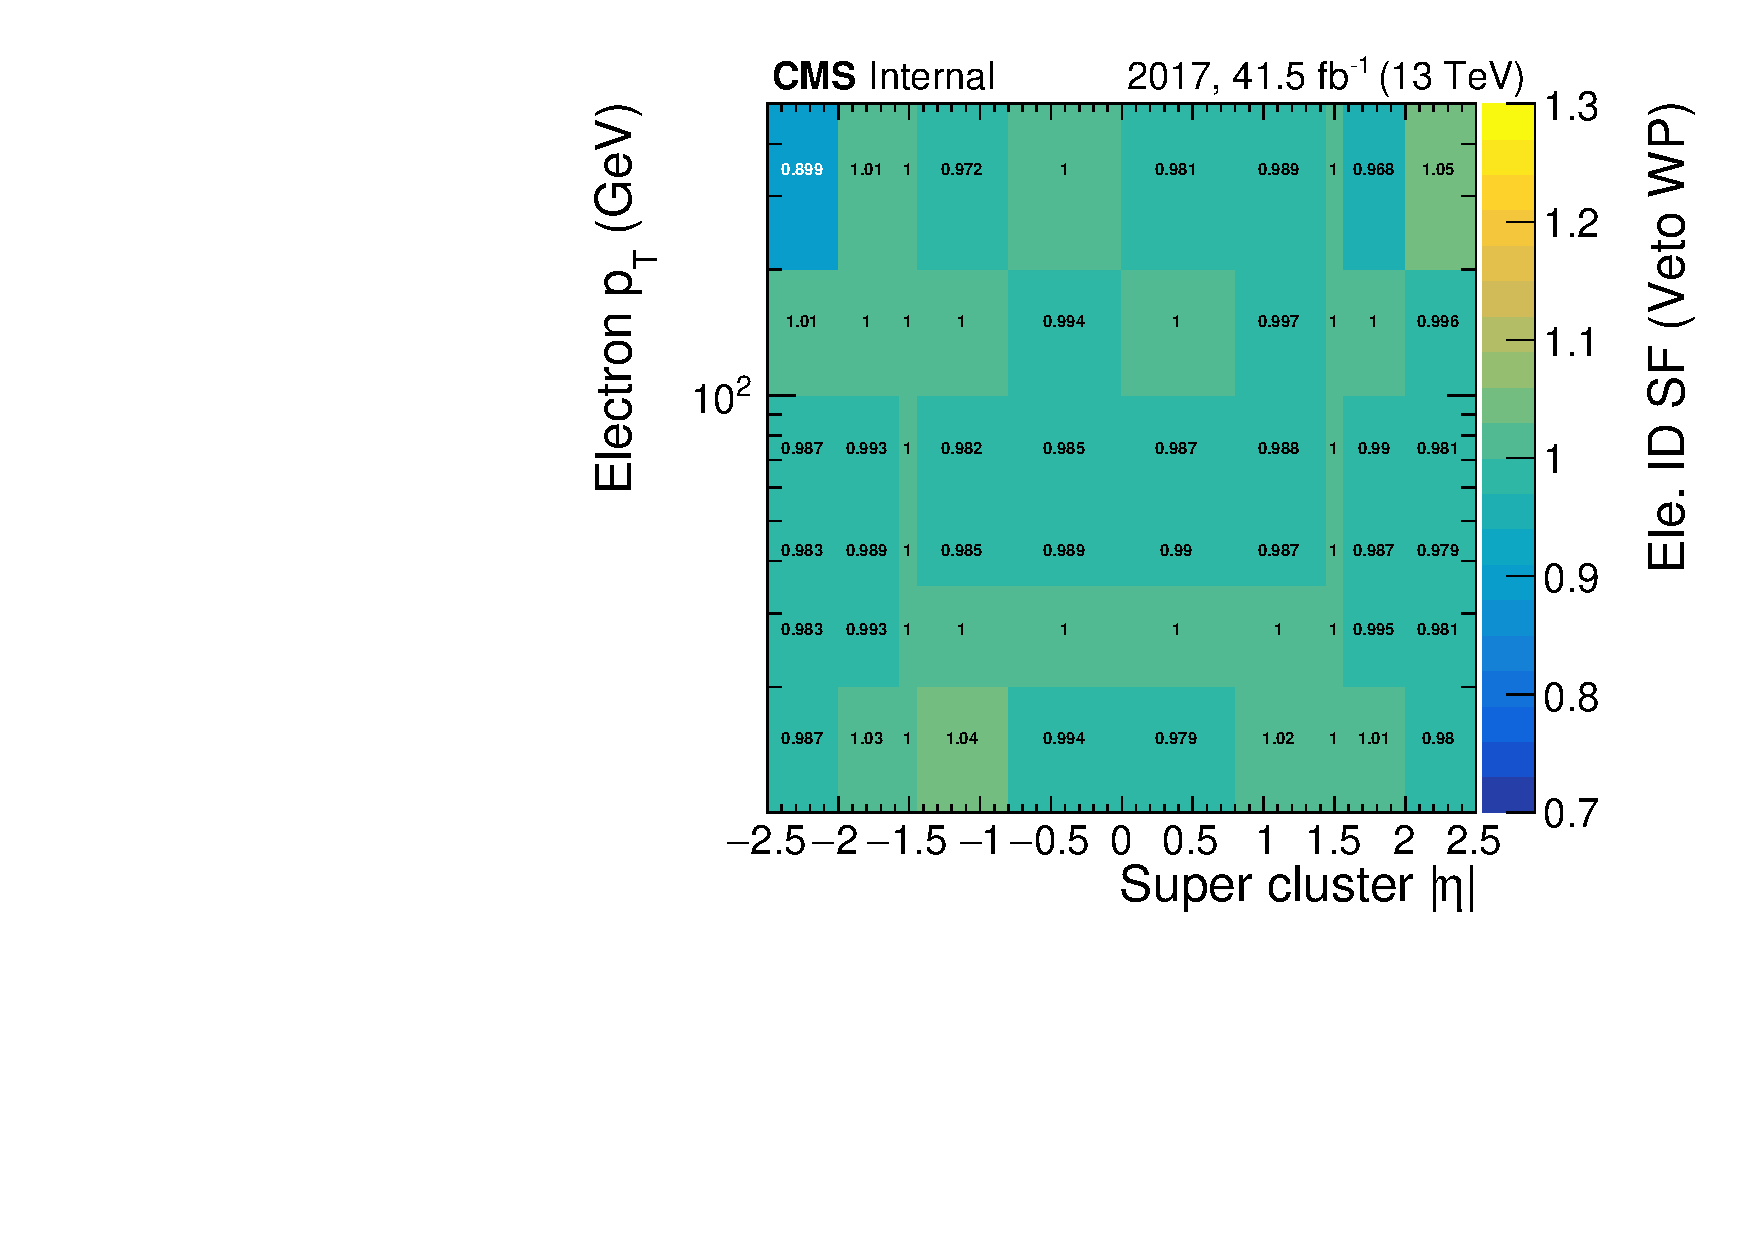
\includegraphics[width=0.49\textwidth]{fig/efficiency/lepton/ele_eff_loose_id_2017.pdf}\\
    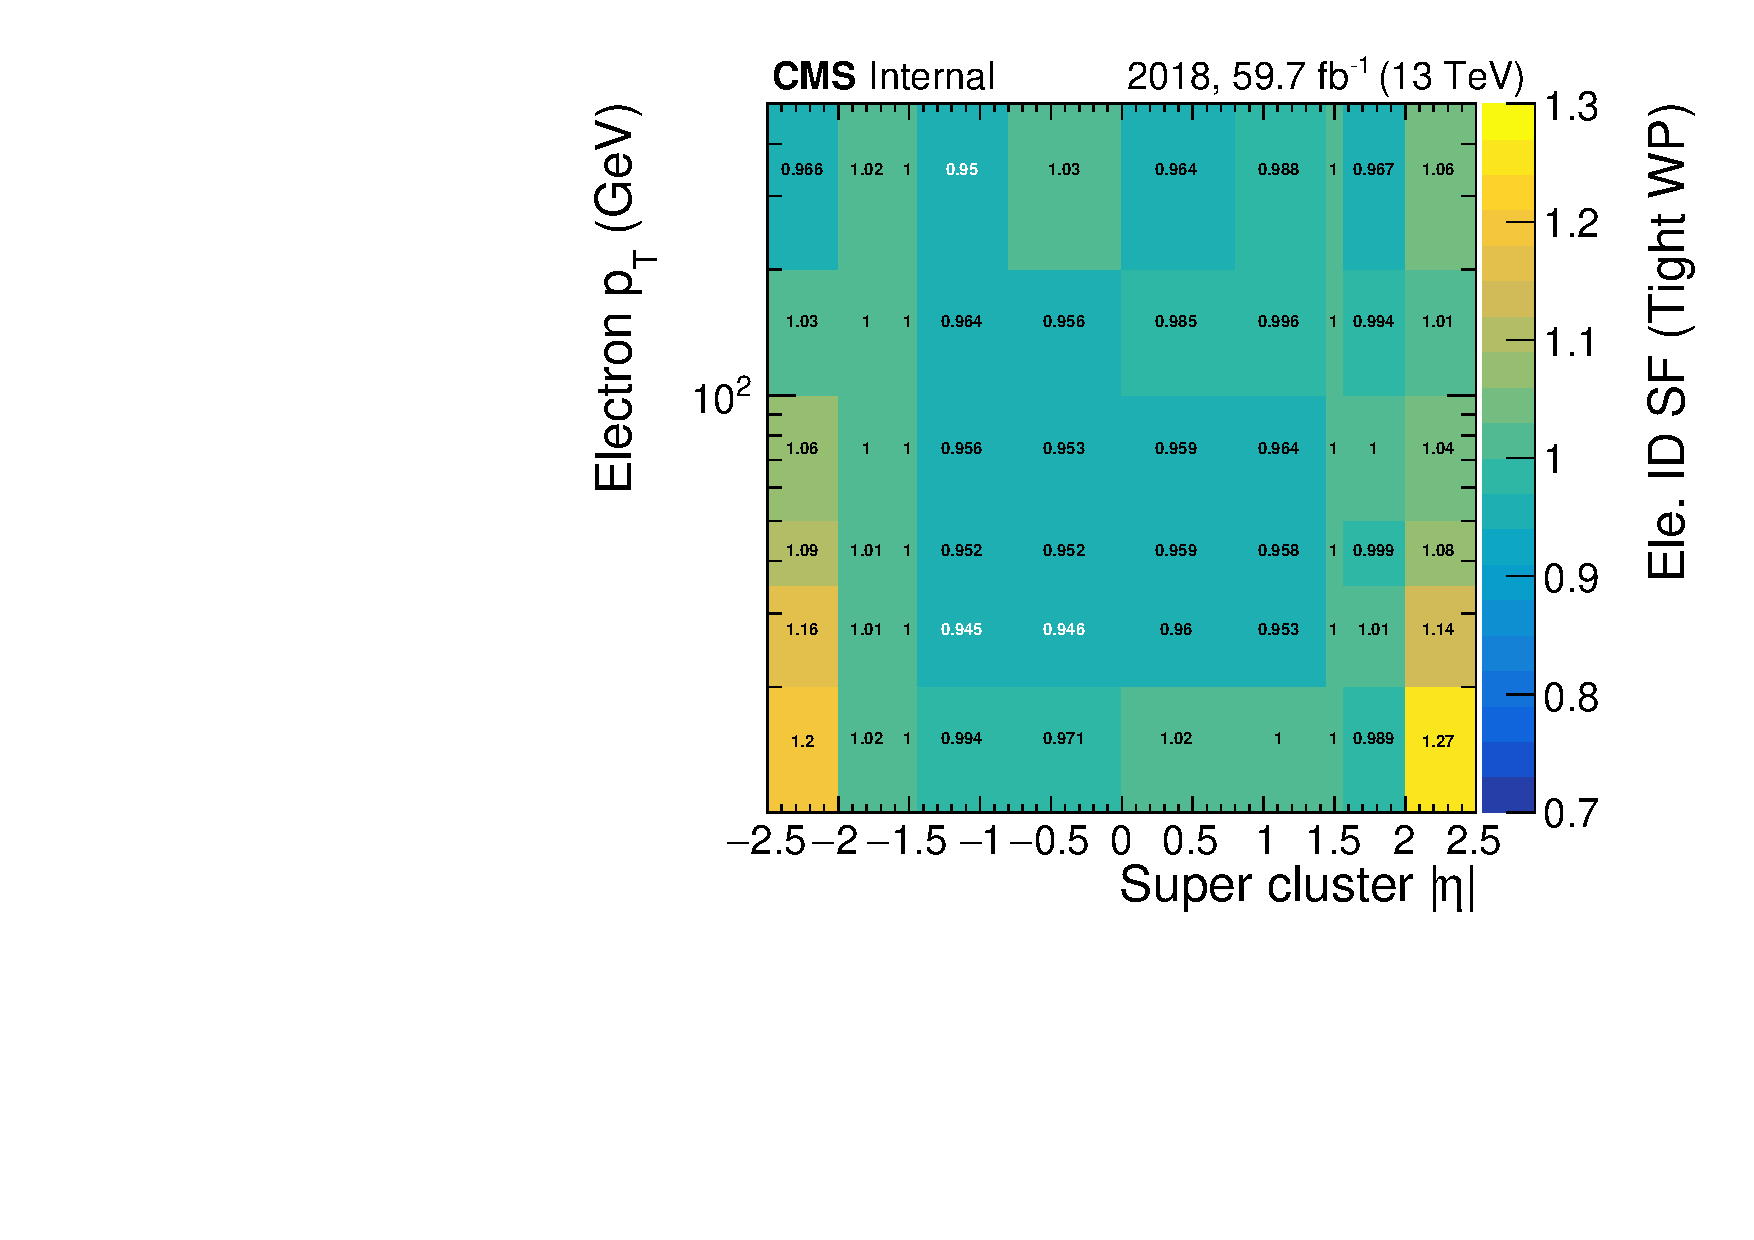
\includegraphics[width=0.49\textwidth]{fig/efficiency/lepton/ele_eff_tight_id_2018.pdf}
    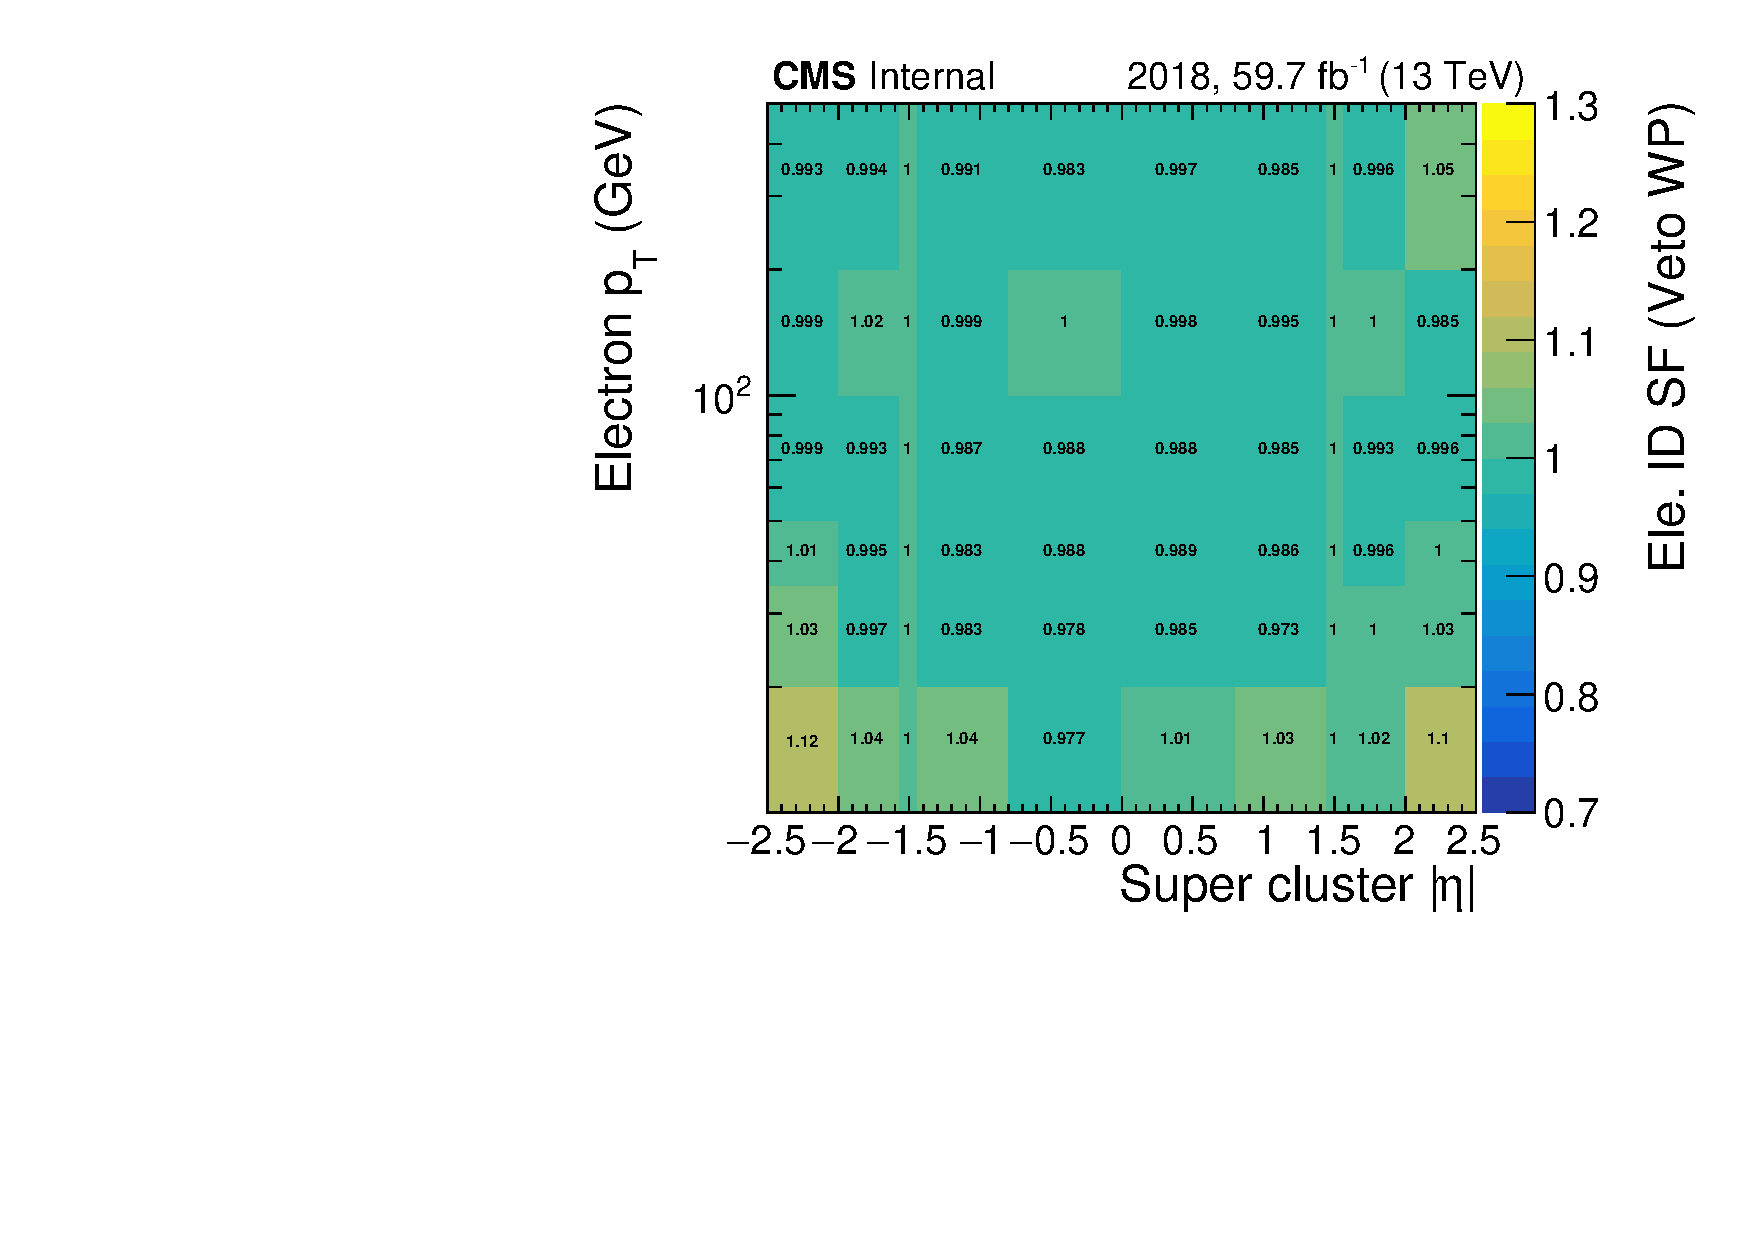
\includegraphics[width=0.49\textwidth]{fig/efficiency/lepton/ele_eff_loose_id_2018.pdf}
    \caption{
      Scale factors for tight (left) and veto (right) electrons are shown for 2017 (top) and
      2018 (bottom). The scale factors are provided in bins of electron $\pt$ and $\eta$.
    }
    \label{fig:sf_electron_id}
  \end{center}
\end{figure}

The scale factors for id and isolation for tight muons are shown in Fig.~\ref{fig:sfmuon}.

\begin{figure}[ht!]
  \begin{center}
    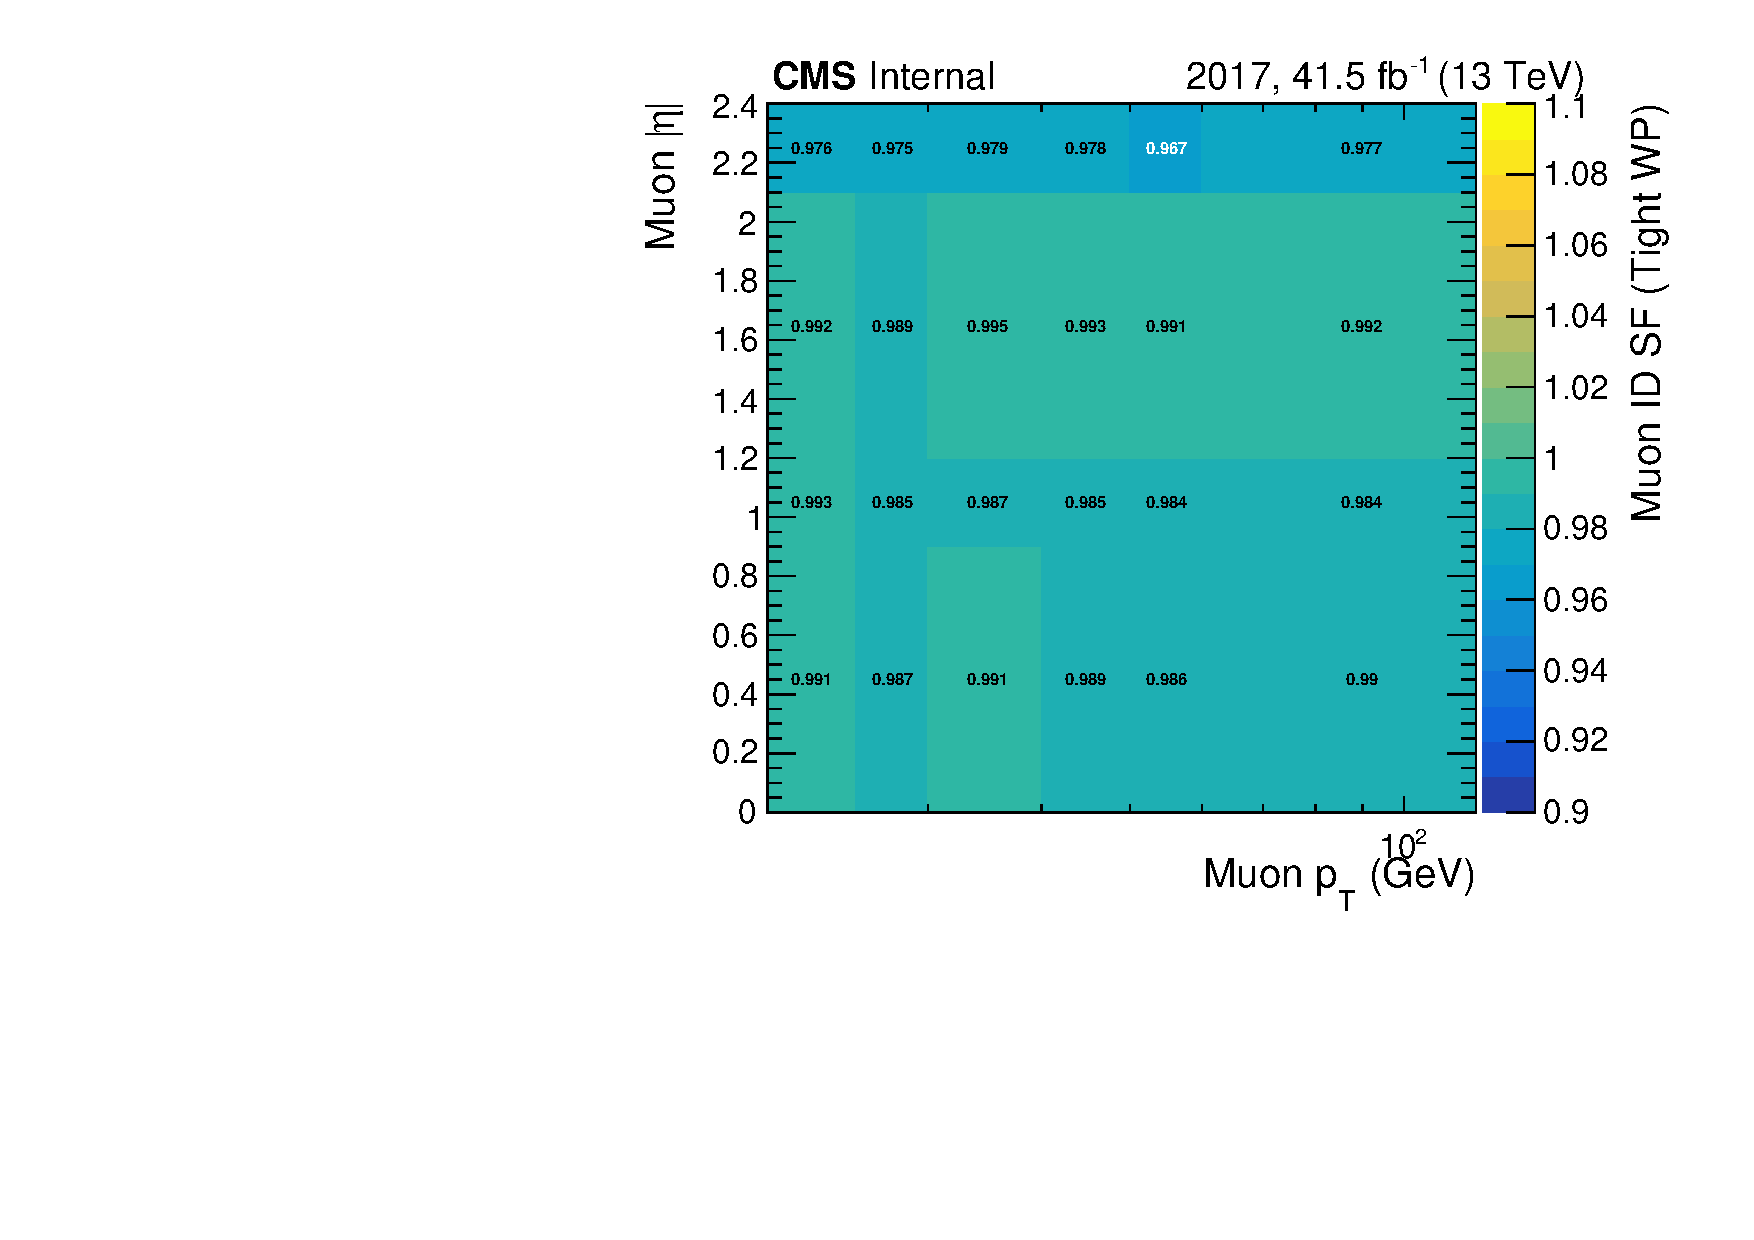
\includegraphics[width=0.49\textwidth]{fig/efficiency/lepton/muon_eff_tight_id_2017.pdf}
    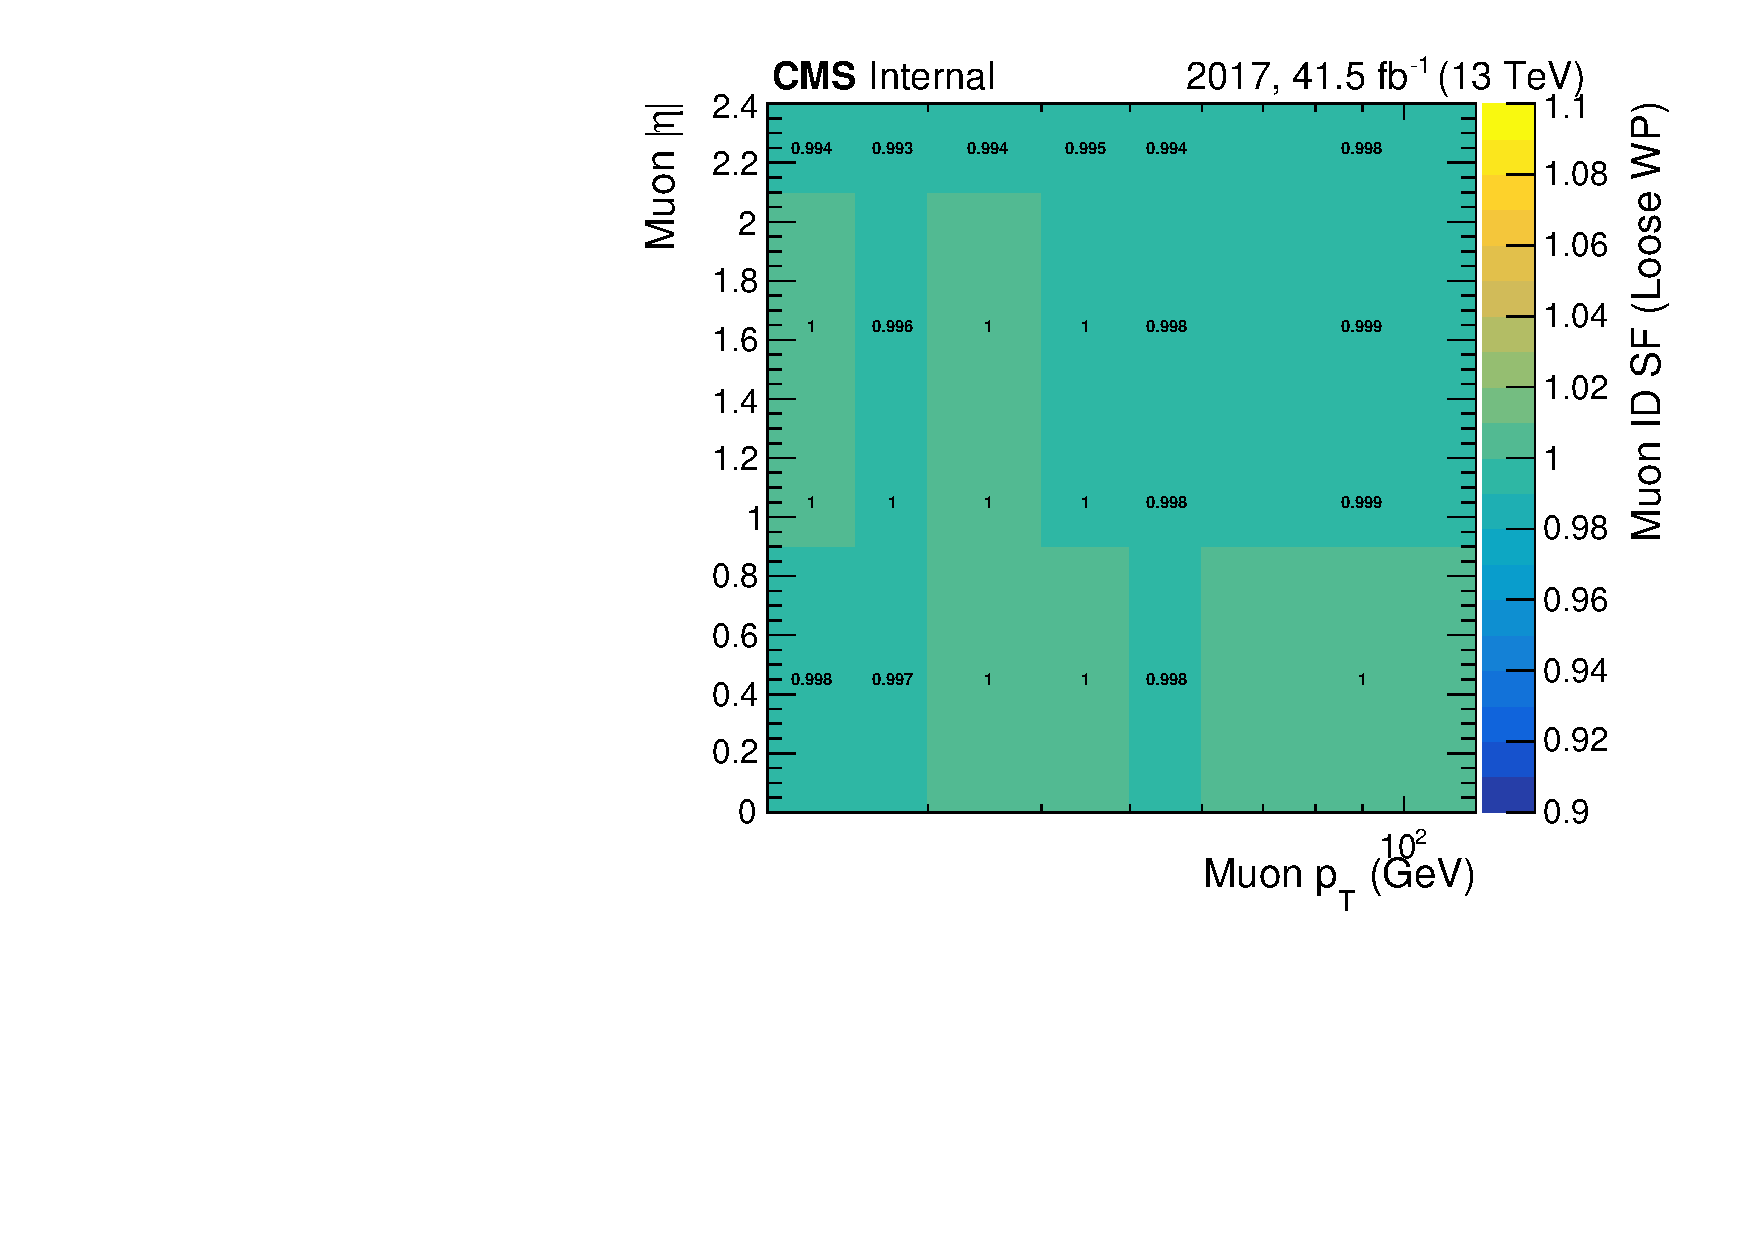
\includegraphics[width=0.49\textwidth]{fig/efficiency/lepton/muon_eff_loose_id_2017.pdf}\\
    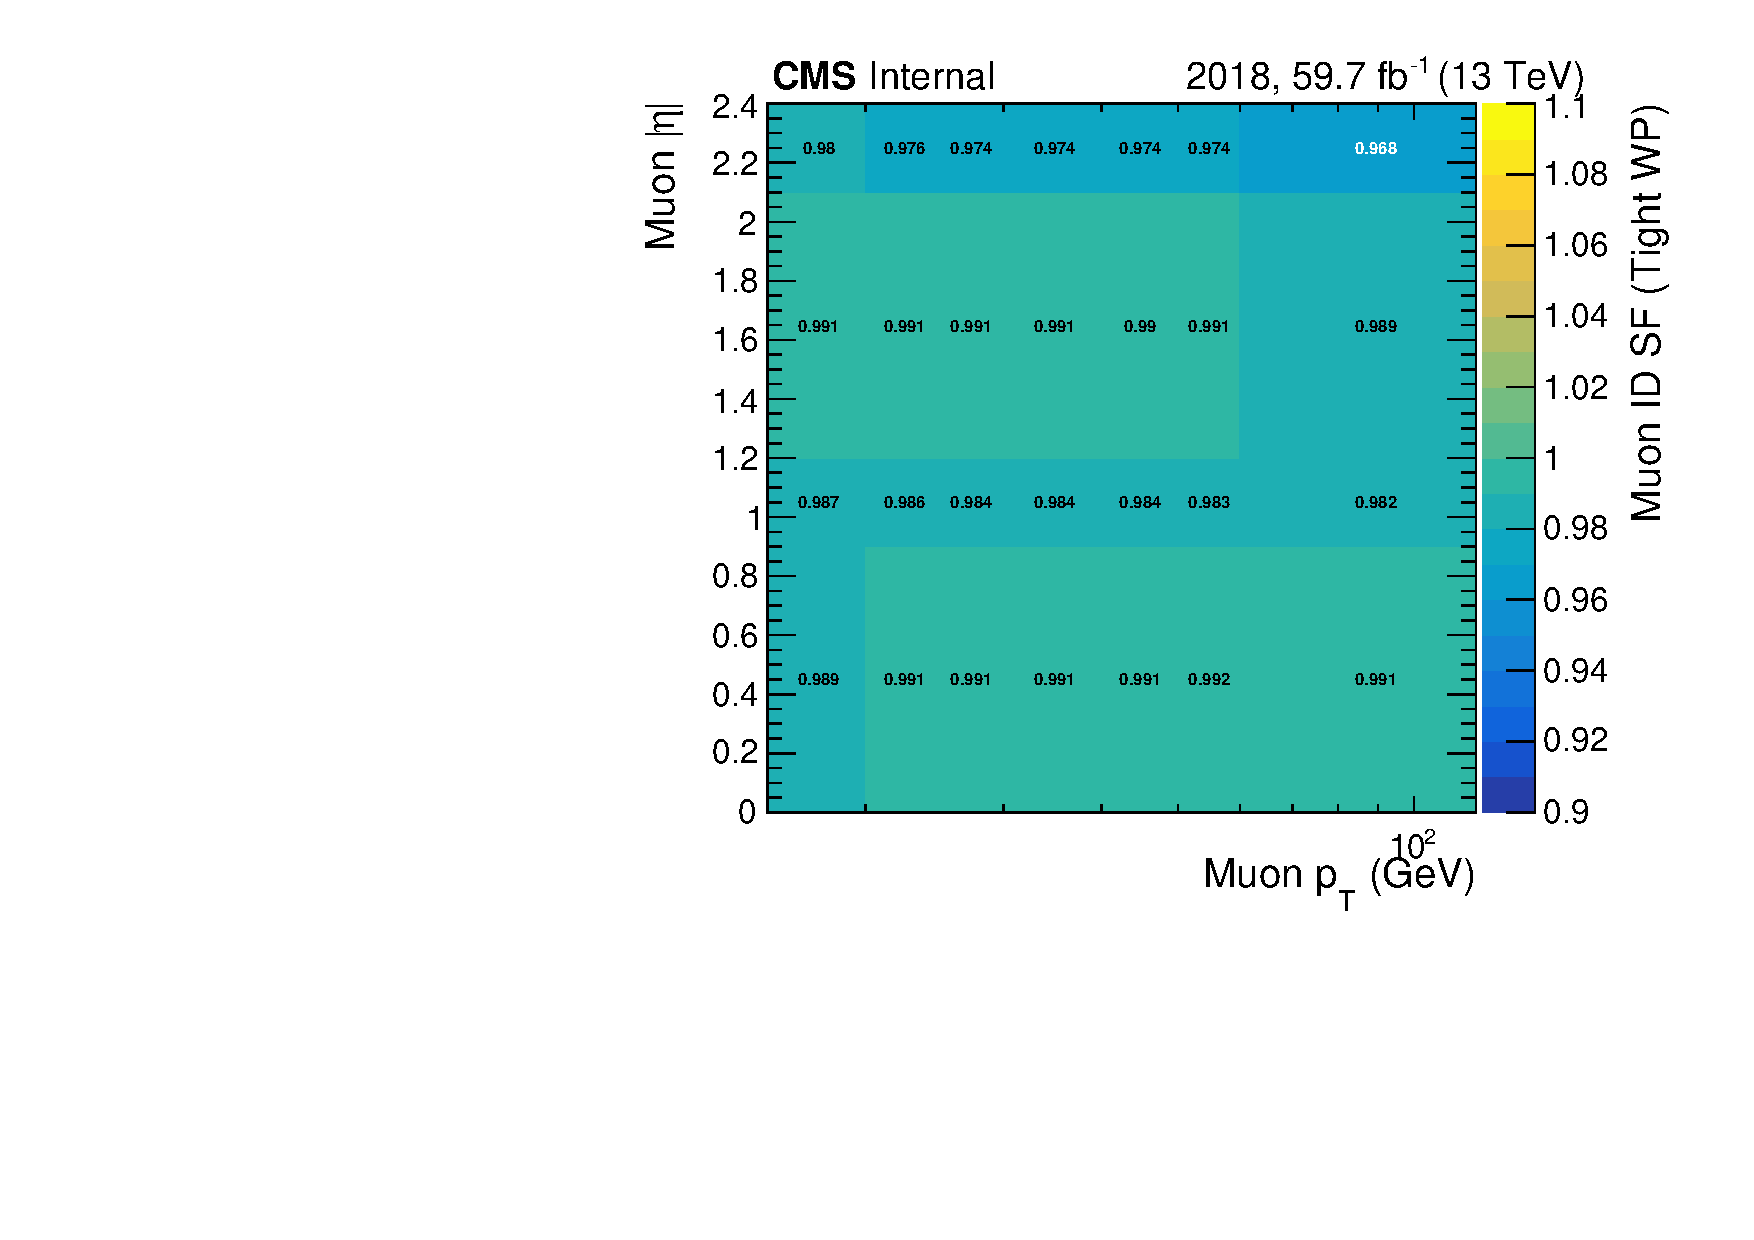
\includegraphics[width=0.49\textwidth]{fig/efficiency/lepton/muon_eff_tight_id_2018.pdf}
    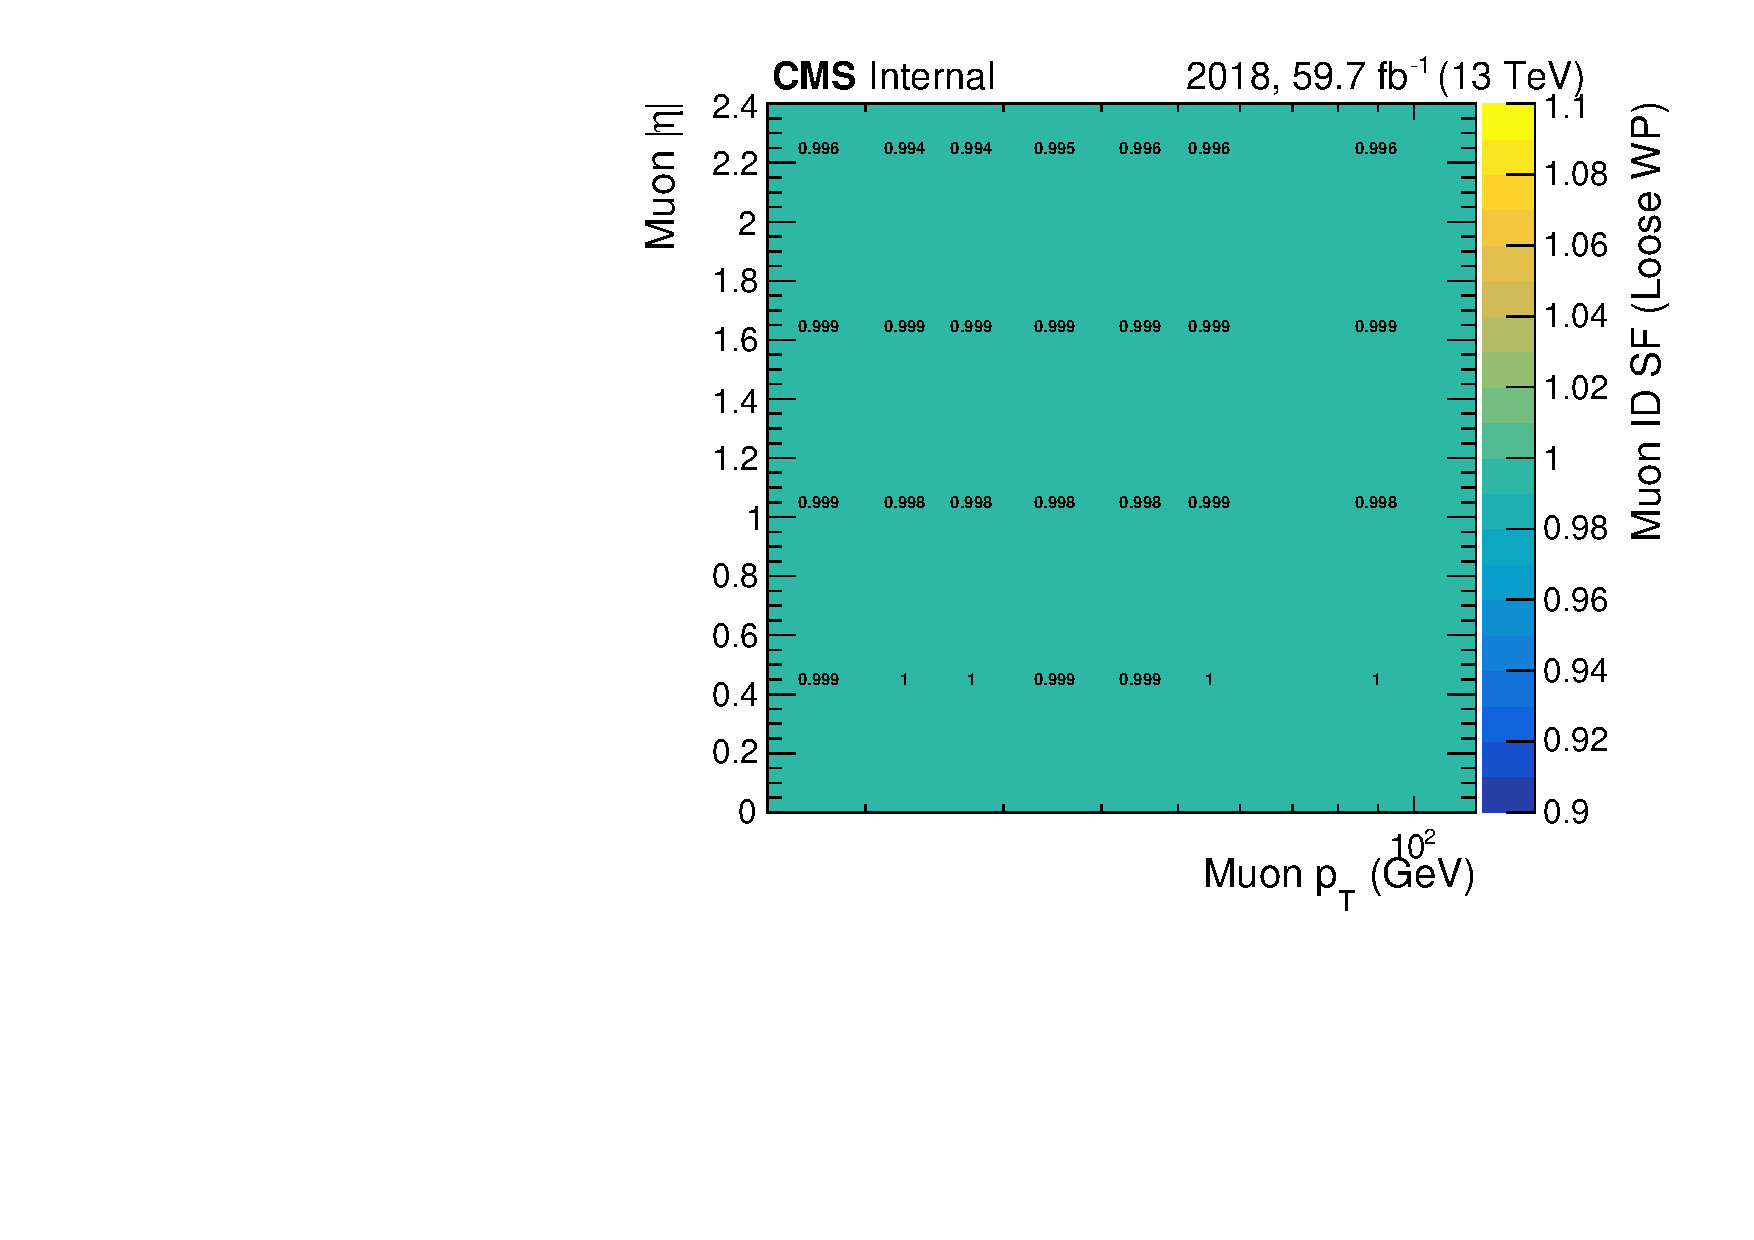
\includegraphics[width=0.49\textwidth]{fig/efficiency/lepton/muon_eff_loose_id_2018.pdf}
    \caption{
      Scale factors for tight (left) and veto (right) muon identification are shown for 2017 (top) and
      2018 (bottom). The scale factors are provided in bins of electron $\pt$ and $\eta$.
    }
    \label{fig:sf_muon_id}
  \end{center}
\end{figure}


\begin{figure}[ht!]
    \begin{center}
        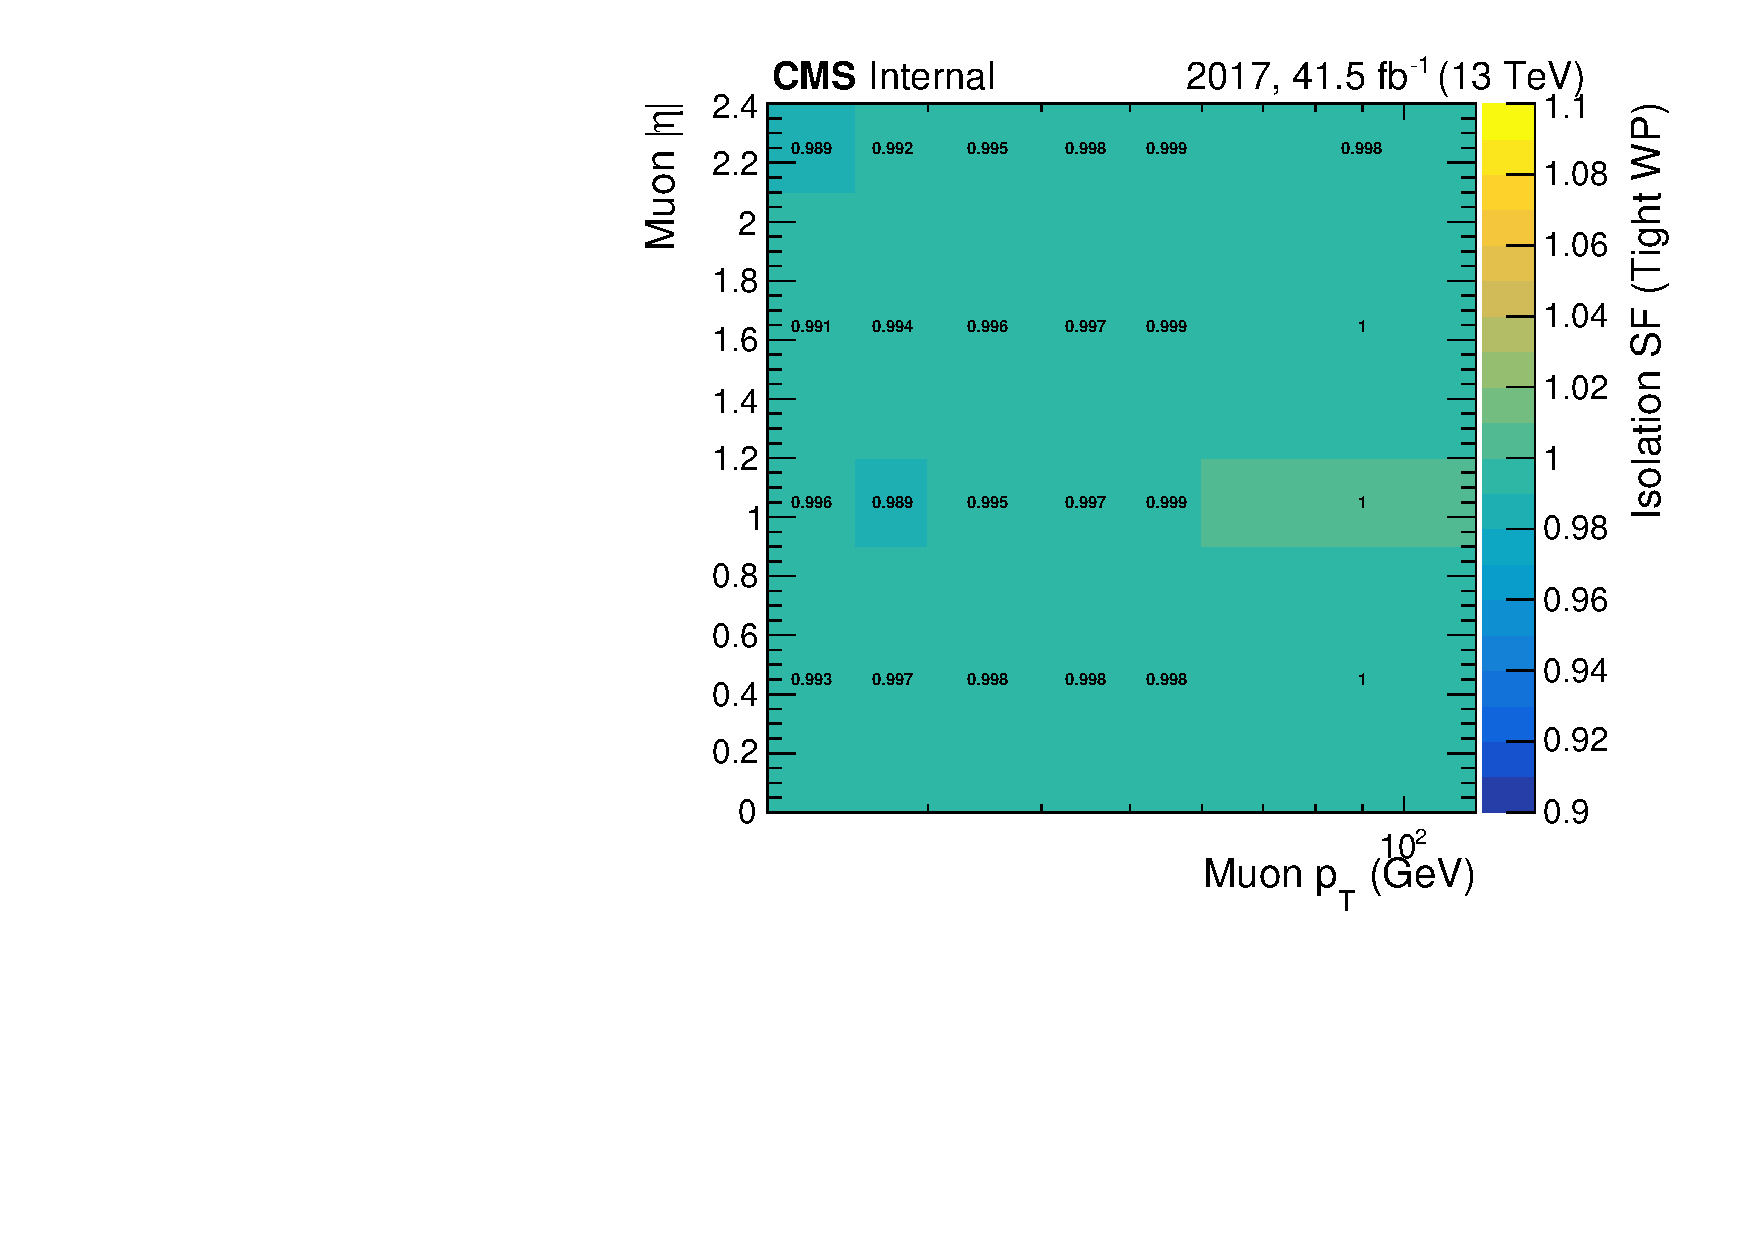
\includegraphics[width=0.49\textwidth]{fig/efficiency/lepton/muon_eff_tight_iso_2017.pdf}
        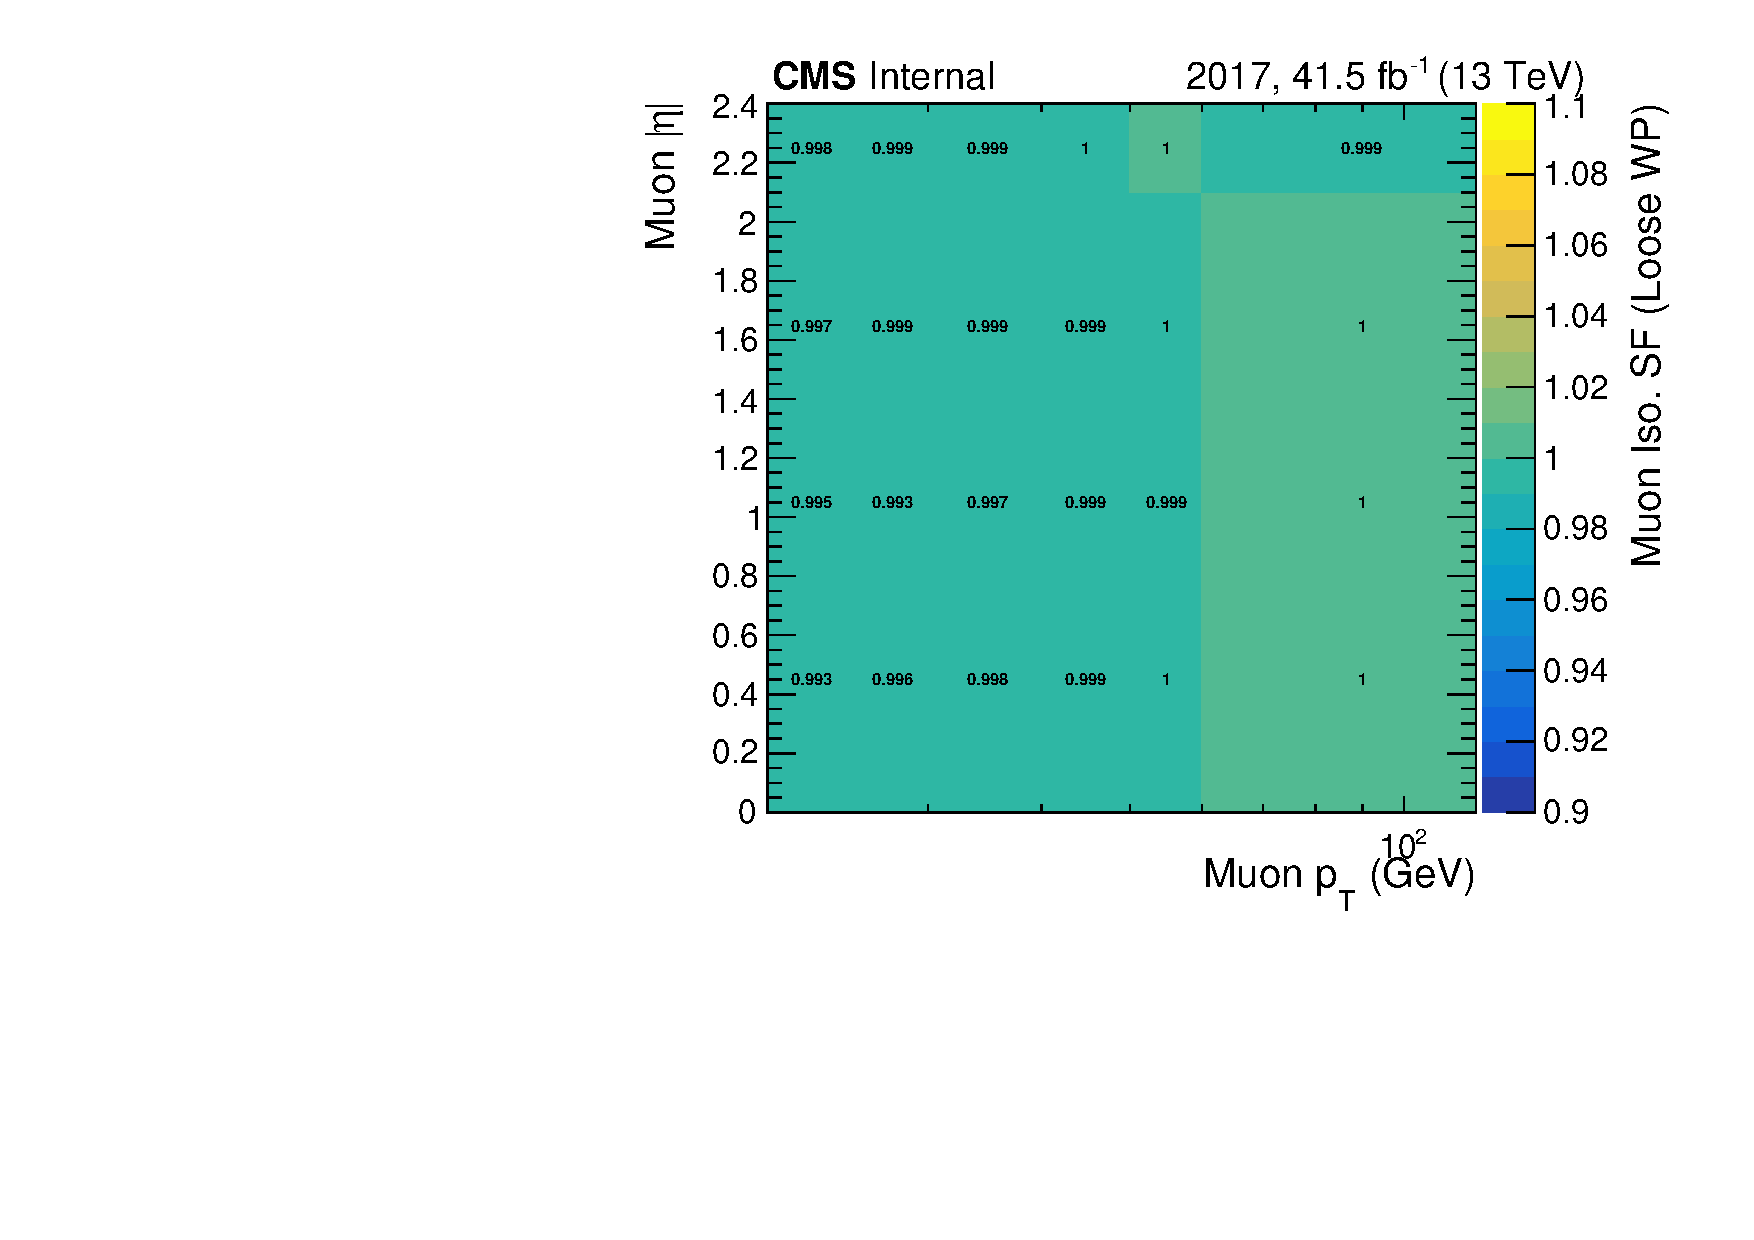
\includegraphics[width=0.49\textwidth]{fig/efficiency/lepton/muon_eff_loose_iso_2017.pdf}\\
        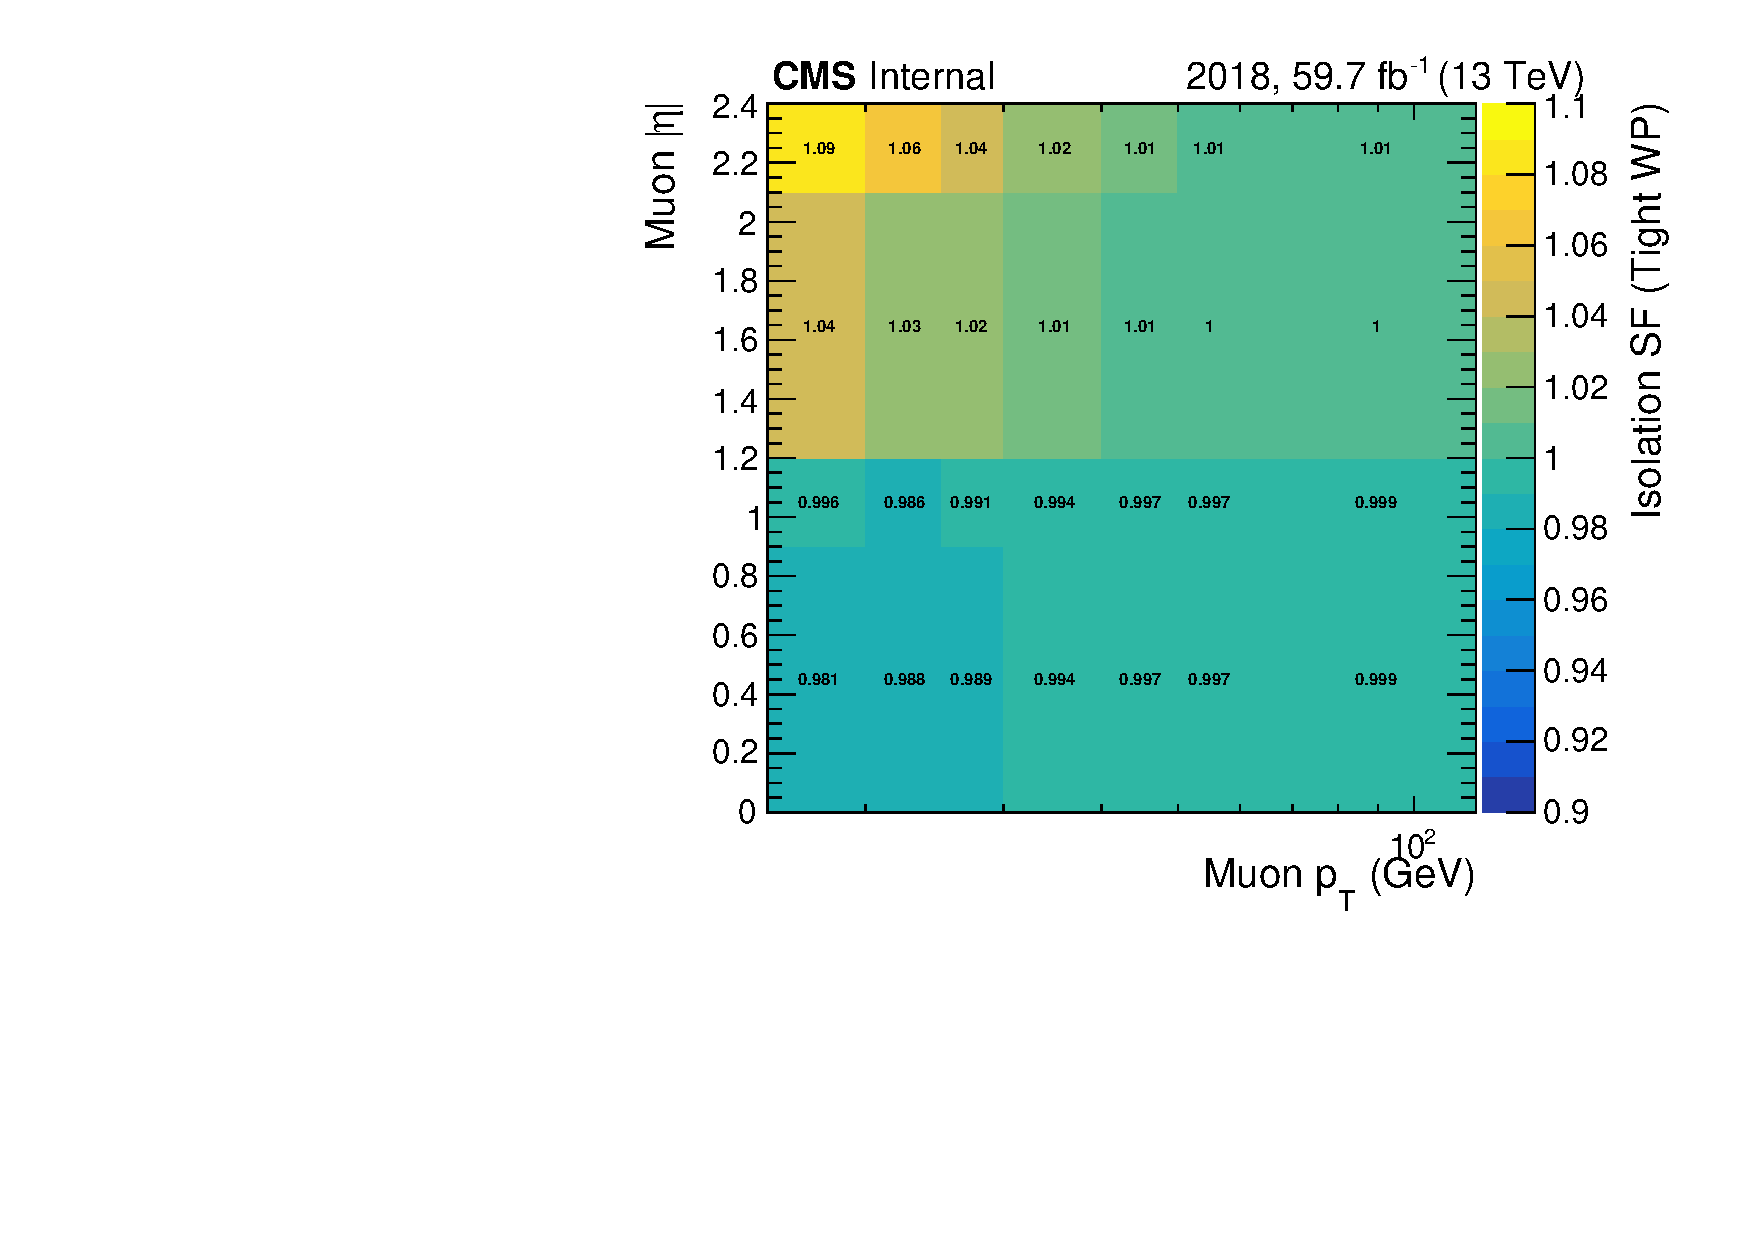
\includegraphics[width=0.49\textwidth]{fig/efficiency/lepton/muon_eff_tight_iso_2018.pdf}
        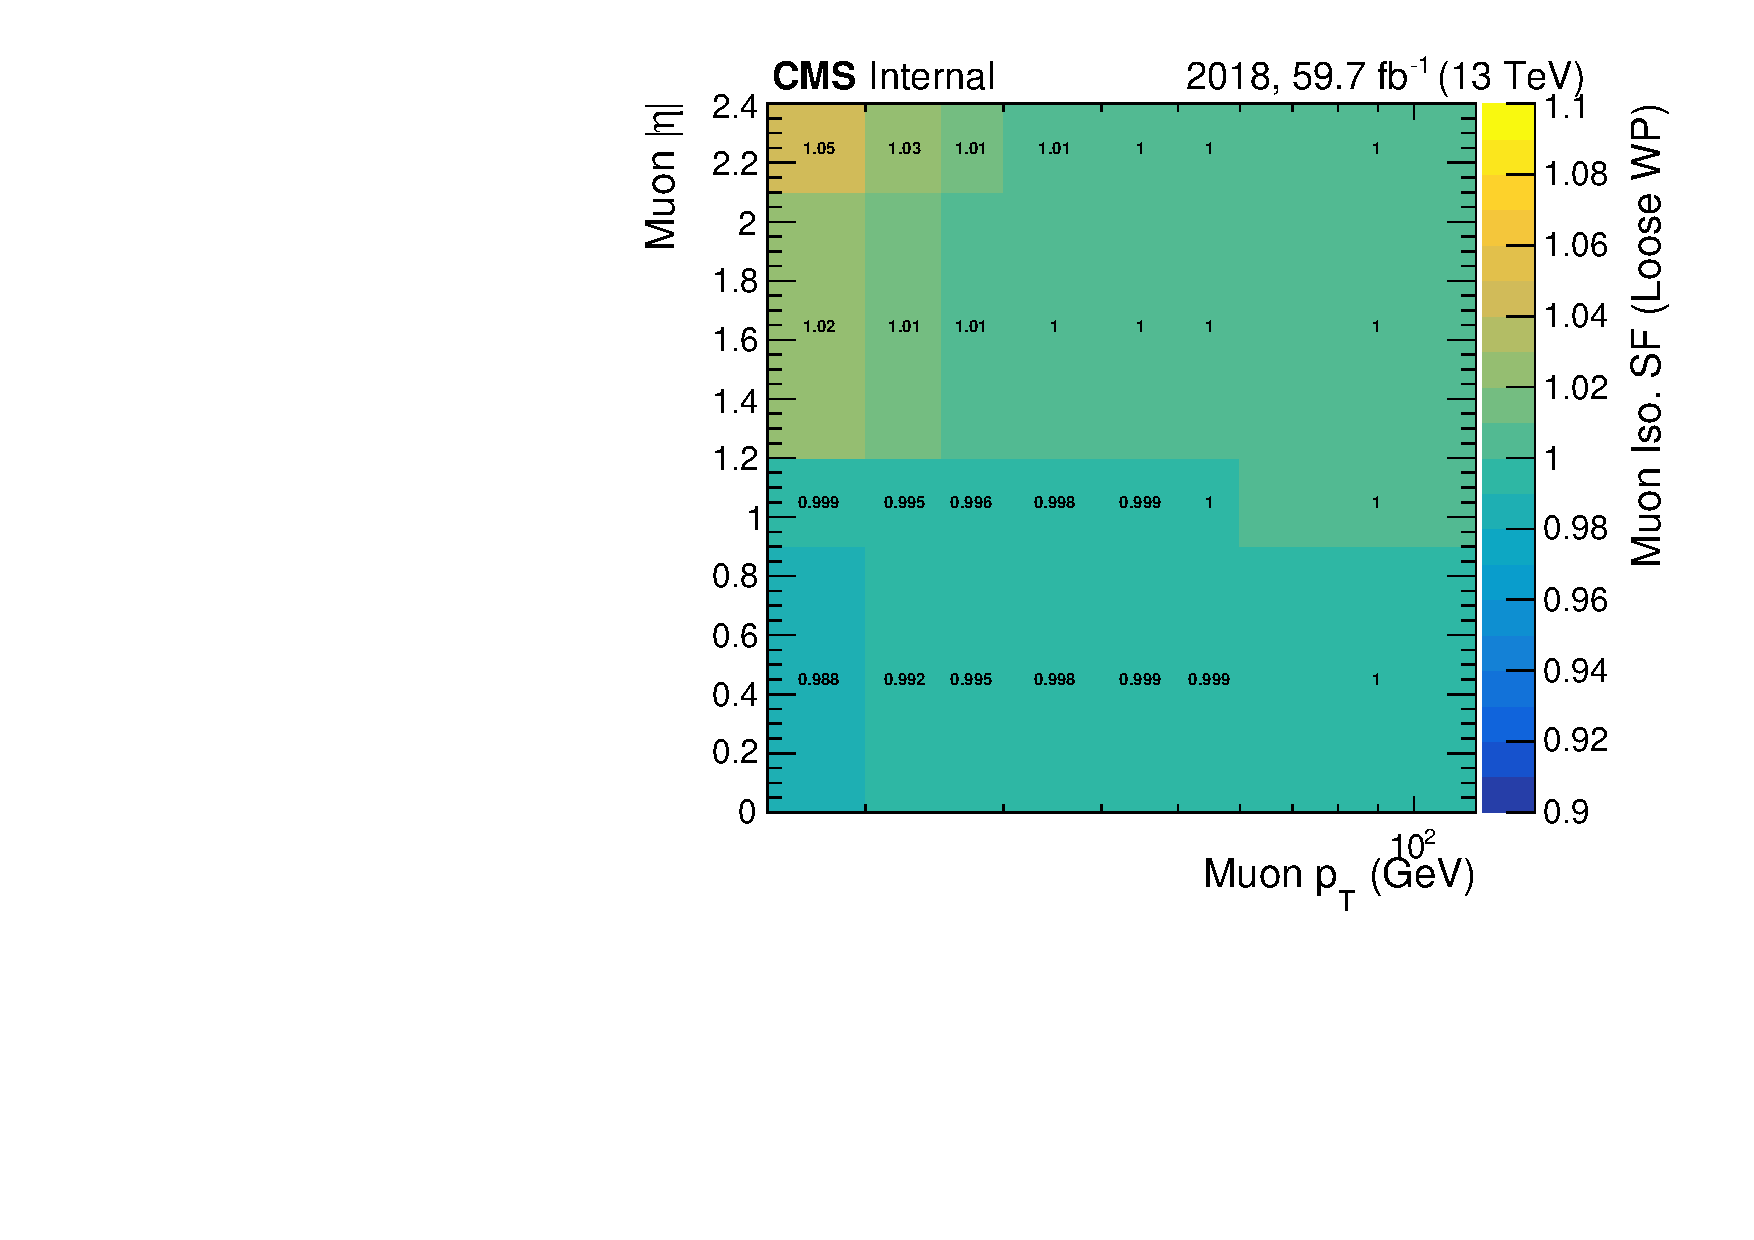
\includegraphics[width=0.49\textwidth]{fig/efficiency/lepton/muon_eff_loose_iso_2018.pdf}
        \caption{
            Scale factors for tight (left) and veto (right) muon isolation are shown for 2017 (top) and
            2018 (bottom). The scale factors are provided in bins of electron $\pt$ and $\eta$.
          }
      \label{fig:sf_muon_iso}
    \end{center}
  \end{figure}

\clearpage
\subsection{Higher-order reweighting}\label{sec:nlo}
This analysis uses the ratios of the recoil distributions in signal and control regions to constrain the final background estimate in a partially data driven way. As signal and control regions both have large statistical power, precise predictions of these ratios are necessary. To achieve this goal, the LO simulation samples for the samples W, DY and photon backgrounds are reweighted using higher-order corrections separately corresponding to NLO QCD, NLO EW and NNLO QCD terms.

\subsubsection{Generator-level boson construction}
All theory-based corrections of the W, DY and photon backgrounds are parametrized as a function of the generator-level \pt of the respective boson \ptv. For each simulated event, this quantity is calculated as follows. For DY and W samples, generator-level dilepton candidates are built from:

\begin{enumerate}
\item ``dressed'' final-state electrons and muons. Lepton dressing means to collect all photons radiated off the lepton within a cone of $\Delta R < 0.1$ and adding their four-momenta back to the lepton four-momentum. This procedure is meant to undo the effect of final state photon radiation, which would otherwise distort the value of the reconstructed boson four-momentum. This effect is especially relevant as electrons and muons follow different radiation patterns. Lepton dressing is performed in central NanoAOD production following the procedure used in the RIVET software.
\item $\tau$ leptons with generator status 2. As $\tau$ leptons are unstable, they are not present as final state particles (status 1) in the generator record. The $\tau$ lepton before its decay has status 2.
\item neutrinos with generator status 1.
\end{enumerate}

The dilepton candidates are checked for flavour consistency with the desired boson candidate. If multiple candidates are found in an event, the one with the highest invariant mass is used.

For photon events, the generator photon with highest \pt and status 1 is used.

\subsubsection{QCD NLO corrections to QCD V processes}

Scale factors corresponding to NLO QCD corrections for W and Z production are obtained from central CMS. For the DY and W processes, samples from ``Fall17'' campaign, while ``Summer16'' samples are used for the $\gamma$+jets process. In both cases, all samples are generated using \texttt{MadGraph5\_amc@NLO}. The LO samples are binned in HT and are equivalent to the ones used in in the analysis, and are generated with up to four partons in the matrix element. The NLO samples are generated with up to two additional partons in the matrix element calculation. Further jet multiplicities are handled by the parton shower, which in both cases is performed using \texttt{Pythia8} with tune \texttt{CP5}.

The scale factors are derived by obtaining the distribution of interest at the generator-level in both samples, normalizing the distributions to their respective cross sections, and then dividing them as SF = NLO / LO. Identical selection criteria are applied to both samples based on the generator-level boson and generator-level AK4 jets, which are clustered using all visible generator particles with status 1. The requirements are:

\begin{enumerate}
\item At least two generator-level jets, with the leading (trailing) \pt of at least 80 GeV (40 GeV) and $|\eta|<4.7$.
\item The two leading jets must be in opposite hemispheres of the detector, $\eta_{1}\times \eta_{2}<0$.
\item The difference in the azimuthal angle ($\Delta\phi$) between the boson and the four leading jets in the event is required to be larger than 0.5. Only jets with $\pt>30~\GeV$ are considered.
\end{enumerate}

Compared to an inclusive derivation of the SF, the inclusion of the selection criteria leads to an increase in the value of the SF of about $10-12\%$.


The scale factors are derived either as a one-dimensional function of the generator-level boson \ptv (``1D'')or two-dimensionally in \ptv and \mjj (``2D'').

The 1D SFs are shown in Fig.~\ref{fig:theory_sf_qcd_nlo}. To protect the outcome of the reweighting procedure from binning effects, the binned scale factor is interpolated using a falling exponential function:
\begin{equation}
\mathtext{SF} = a\times \exp(-b\times\pt) + c,
\end{equation}

where \pt is the boson transverse momentum and a, b and c are determined by a fit to the scale factor histogram. The resulting values of the fit parameters, as well as the resulting interpolated shape are also shown in Fig.~\ref{fig:theory_sf_qcd_nlo}.

The 2D versions of the SFs are only derived for the W and DY processes, for which the available simulation samples are bigger and thus allow for finer binning. The scale factors are shown in Fig.~\ref{fig:theory_sf_qcd_nlo_2d}.


\begin{figure}[ht!]
    \begin{center}
        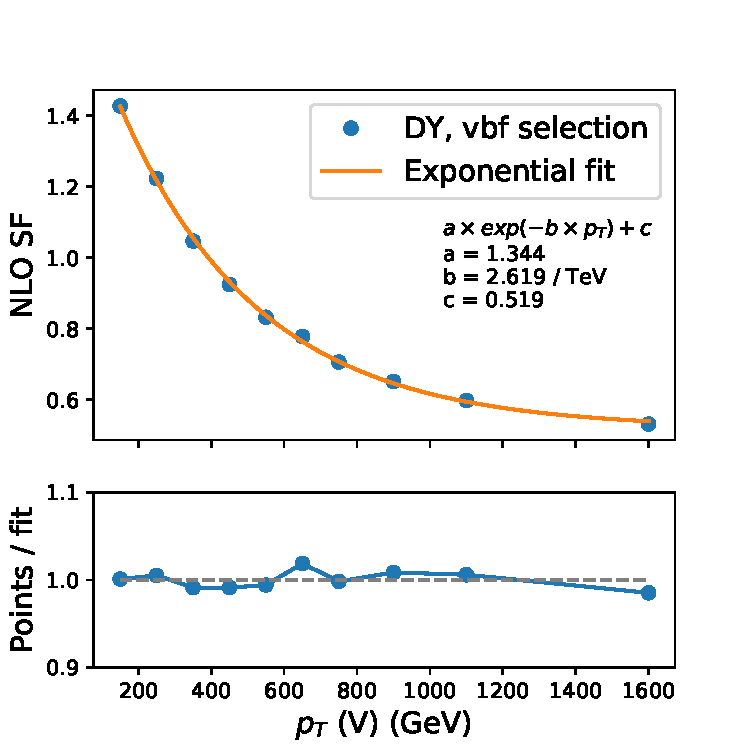
\includegraphics[width=0.49\textwidth]{fig/theory/interpolation_vbf_dy.pdf}
        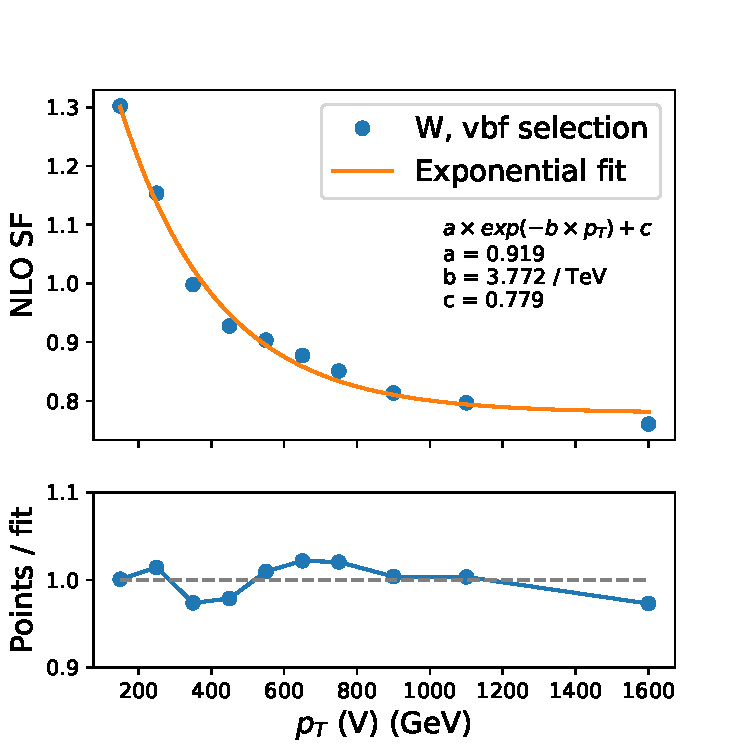
\includegraphics[width=0.49\textwidth]{fig/theory/interpolation_vbf_wjet.pdf} \\
        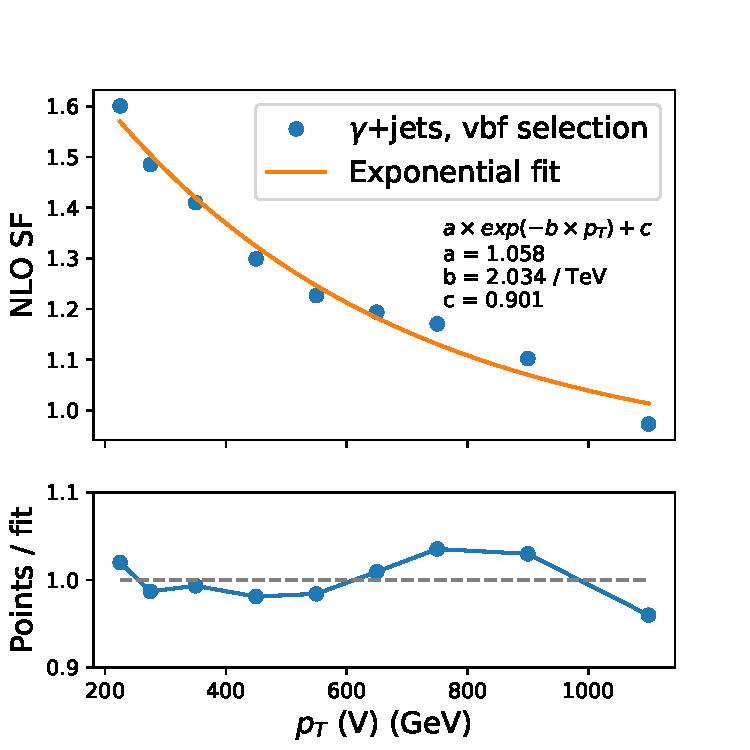
\includegraphics[width=0.49\textwidth]{fig/theory/interpolation_vbf_gjets.pdf}
        \caption{
            QCD NLO scale factors for the DY (top left), W (top right) and $\gamma$+jets processes.
            The k factors are derived within the generator-level VBF selection described in the text.
            In the top panel of each plot, the blue markers show the NLO SF derived from the simulated samples. The orange line shows a fit function used
            to interpolate the SF. The functional form and resulting parameters are given in the figure. In the bottom panel, the blue markers
            show the ratio of the histogram to the fit result in each bin.
          }
      \label{fig:theory_sf_qcd_nlo}
    \end{center}
  \end{figure}

\begin{figure}[ht!]
    \begin{center}
        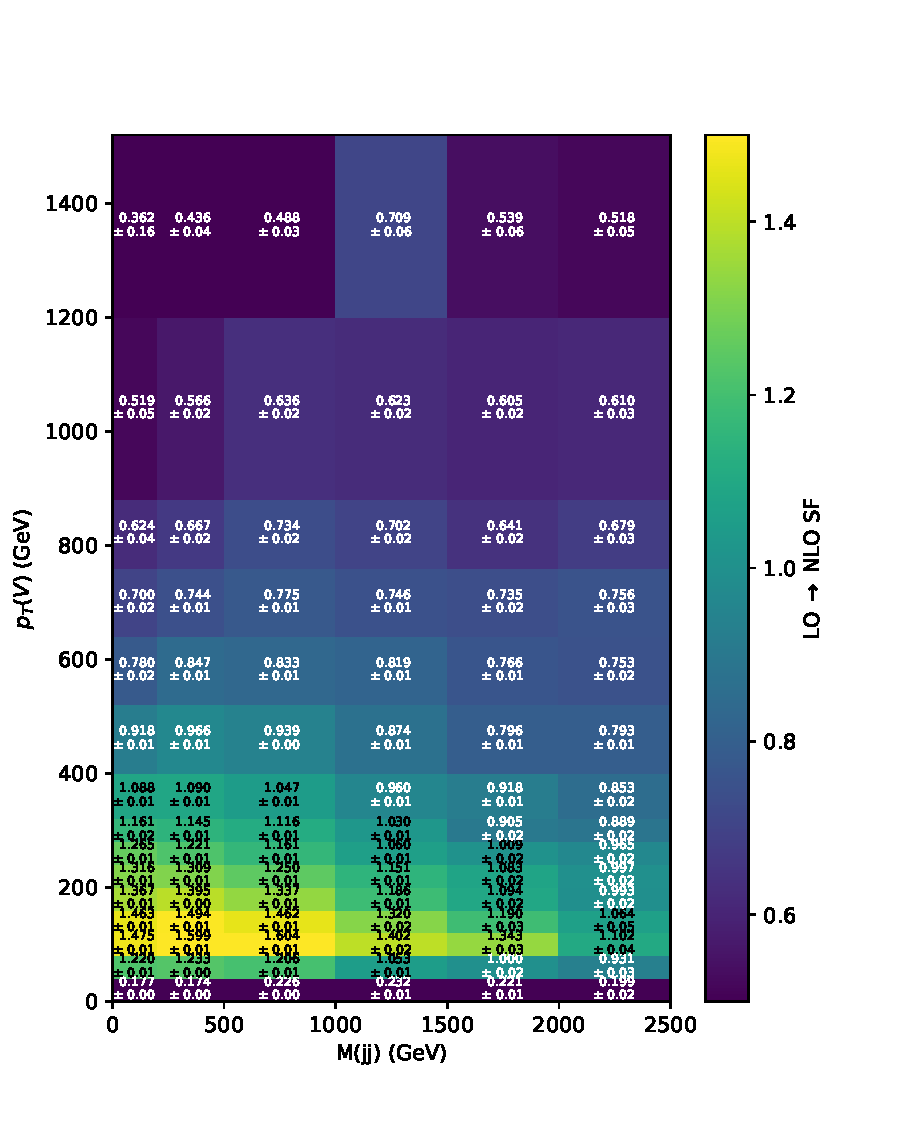
\includegraphics[width=0.49\textwidth]{fig/theory/2d_dy_gen_vpt_vbf_dress.pdf}
        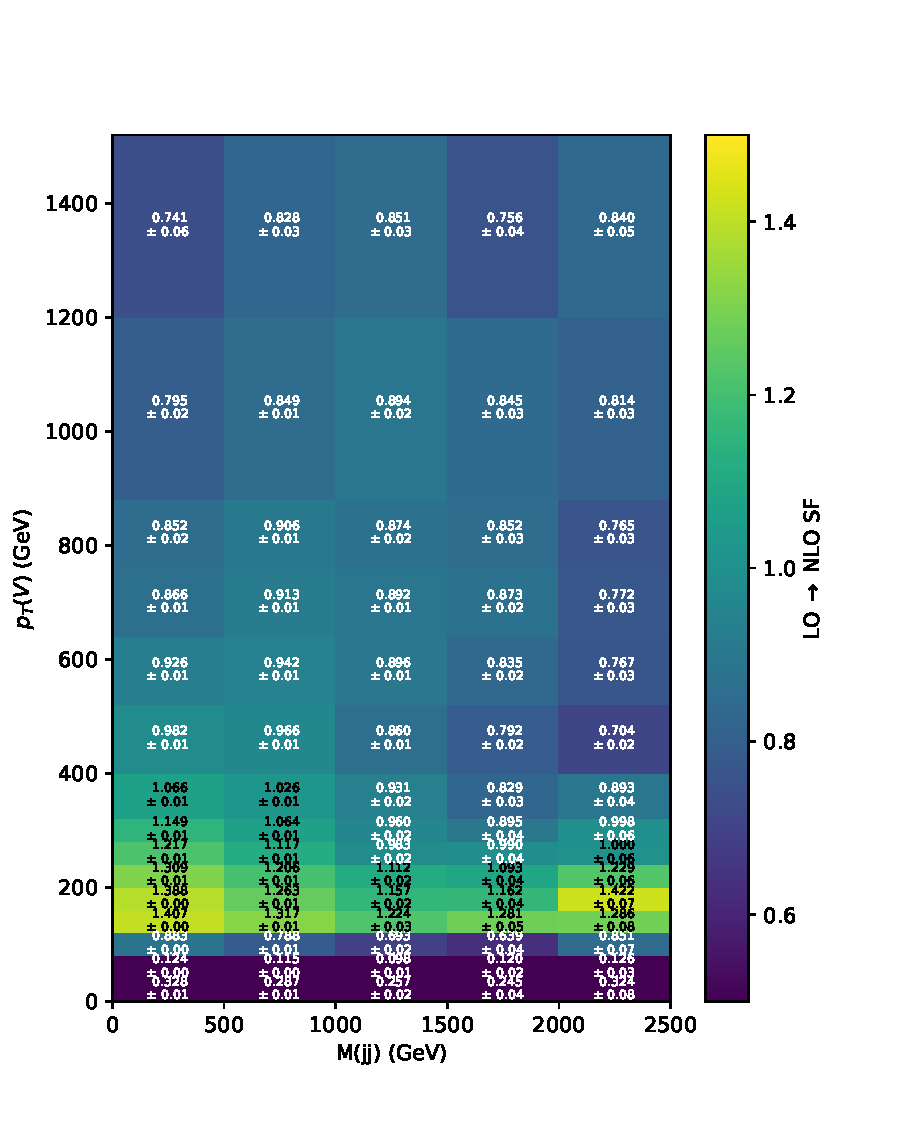
\includegraphics[width=0.49\textwidth]{fig/theory/2d_wjet_gen_vpt_vbf_dress.pdf} \\
        \caption{
            Same as Fig.~\ref{fig:theory_sf_qcd_nlo}, but now binned in two dimensions of the generator-level boson \pt and \mjj.
            The k factors are derived within the generator-level VBF selection described in the text.
            The uncertainties quoted in each bin are the statistical uncertainties due to the finite size of simulated samples.
          }
      \label{fig:theory_sf_qcd_nlo_2d}
    \end{center}
  \end{figure}

\subsubsection{QCD NNLO corrections to QCD V processes}

NNLO corrections are obtained from the fixed-order calculations results in~\ref{DMTheory}. They are parametrized as a function of the generator-level boson \pt. The correction is shown in Fig.~\ref{fig:theory_sf_qcd_nnlo}.

\begin{figure}[ht!]
    \begin{center}
        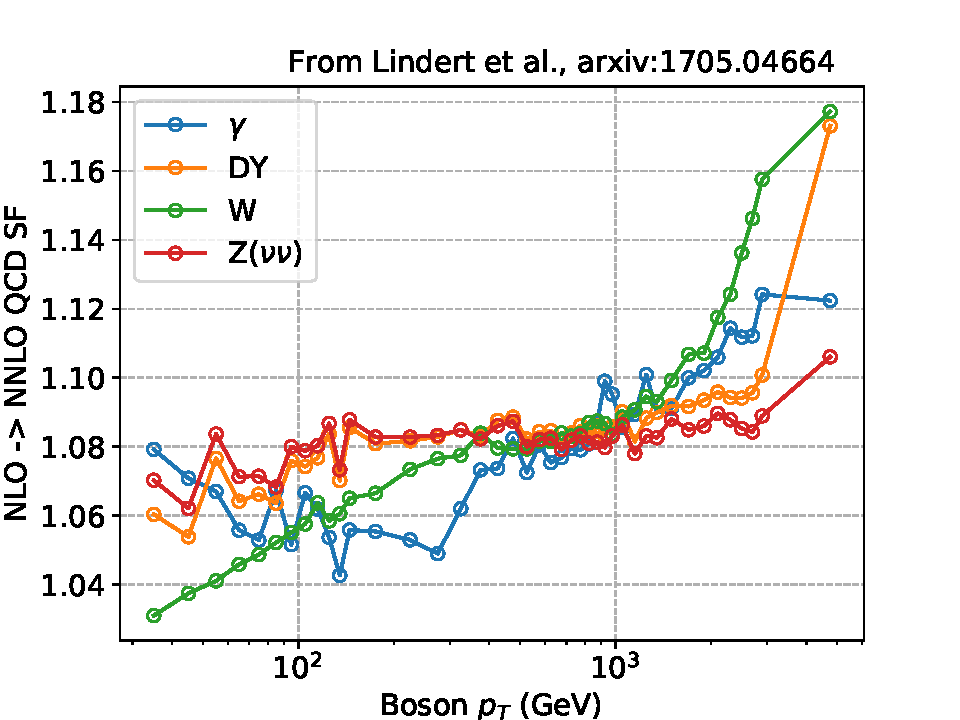
\includegraphics[width=0.49\textwidth]{fig/theory/nnlo_qcd.pdf}
        \caption{
            QCD NNLO scale factors for DY, W and photon production as a function of \ptv.
          }
      \label{fig:theory_sf_qcd_nnlo}
    \end{center}
  \end{figure}

\subsubsection{EW NLO corrections to QCD V processes}
Scale factors corresponding to NLO EW corrections are obtained from Ref.~\cite{DMTheory} and applied as a function of the generator-level boson \pt. The scale factors are shown in Fig.~\ref{fig:theory_sf_ew_nlo}.

\begin{figure}[ht!]
    \begin{center}
        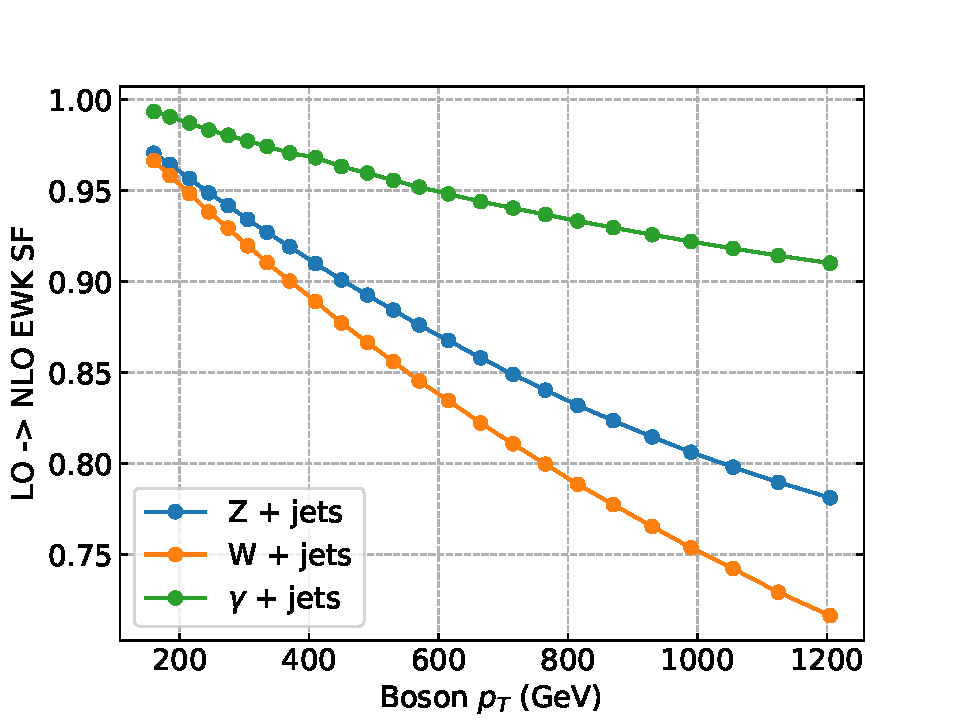
\includegraphics[width=0.49\textwidth]{fig/theory/ewnlo/nlo_ewk.pdf}
        \caption{
            EW NLO scale factors for DY, W and photon production as a function of \ptv.
          }
      \label{fig:theory_sf_ew_nlo}
    \end{center}
  \end{figure}

\subsubsection{QCD NLO corrections to EWK V processes}
The QCD NLO corrections to EWK W and Z production have been calculated in Ref.~\cite{AN-2017-267} using the VBF@NLO program. They are parametrized in \ptv and \mjj and are shown in Fig.~\ref{fig:theory_sf_ew_nlo}.


\begin{figure}[ht!]
    \begin{center}
        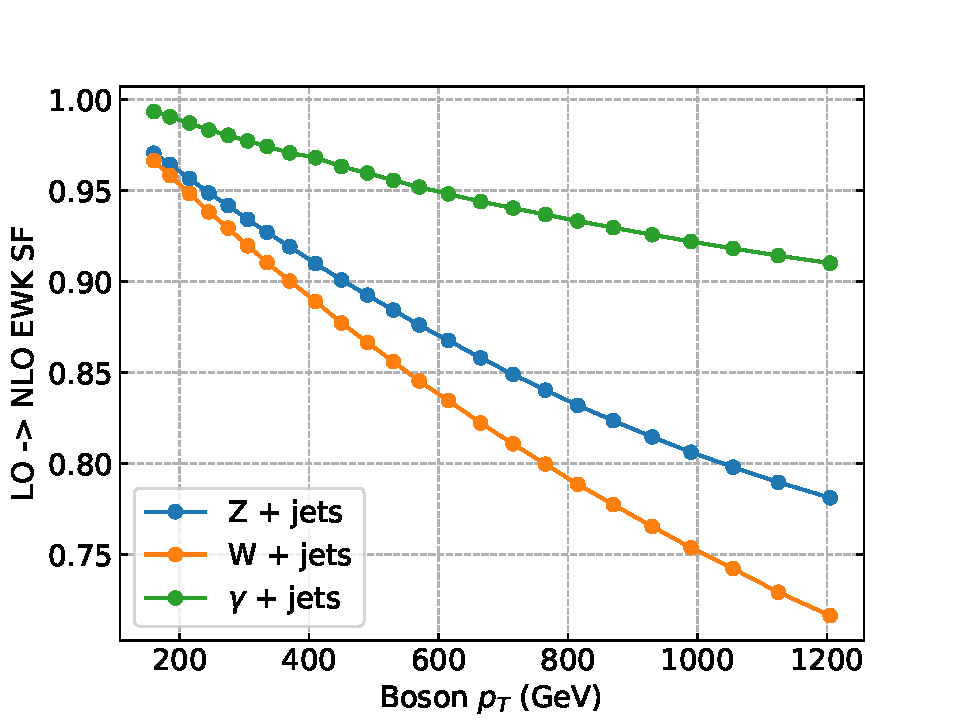
\includegraphics[width=0.49\textwidth]{fig/theory/ewnlo/nlo_ewk.pdf}
        \caption{
            EW NLO scale factors for DY, W and photon production as a function of \ptv.
          }
      \label{fig:theory_sf_ew_nlo}
    \end{center}
  \end{figure}